\chapter{Gráficos de resultados numéricos capítulo 3}

\section{A}


\chapter{Gráficos de resultados numéricos capítulo 4}

\subsection{}

\begin{figure}[h!]
    \centering
    \begin{subfigure}[b]{0.49\textwidth}
        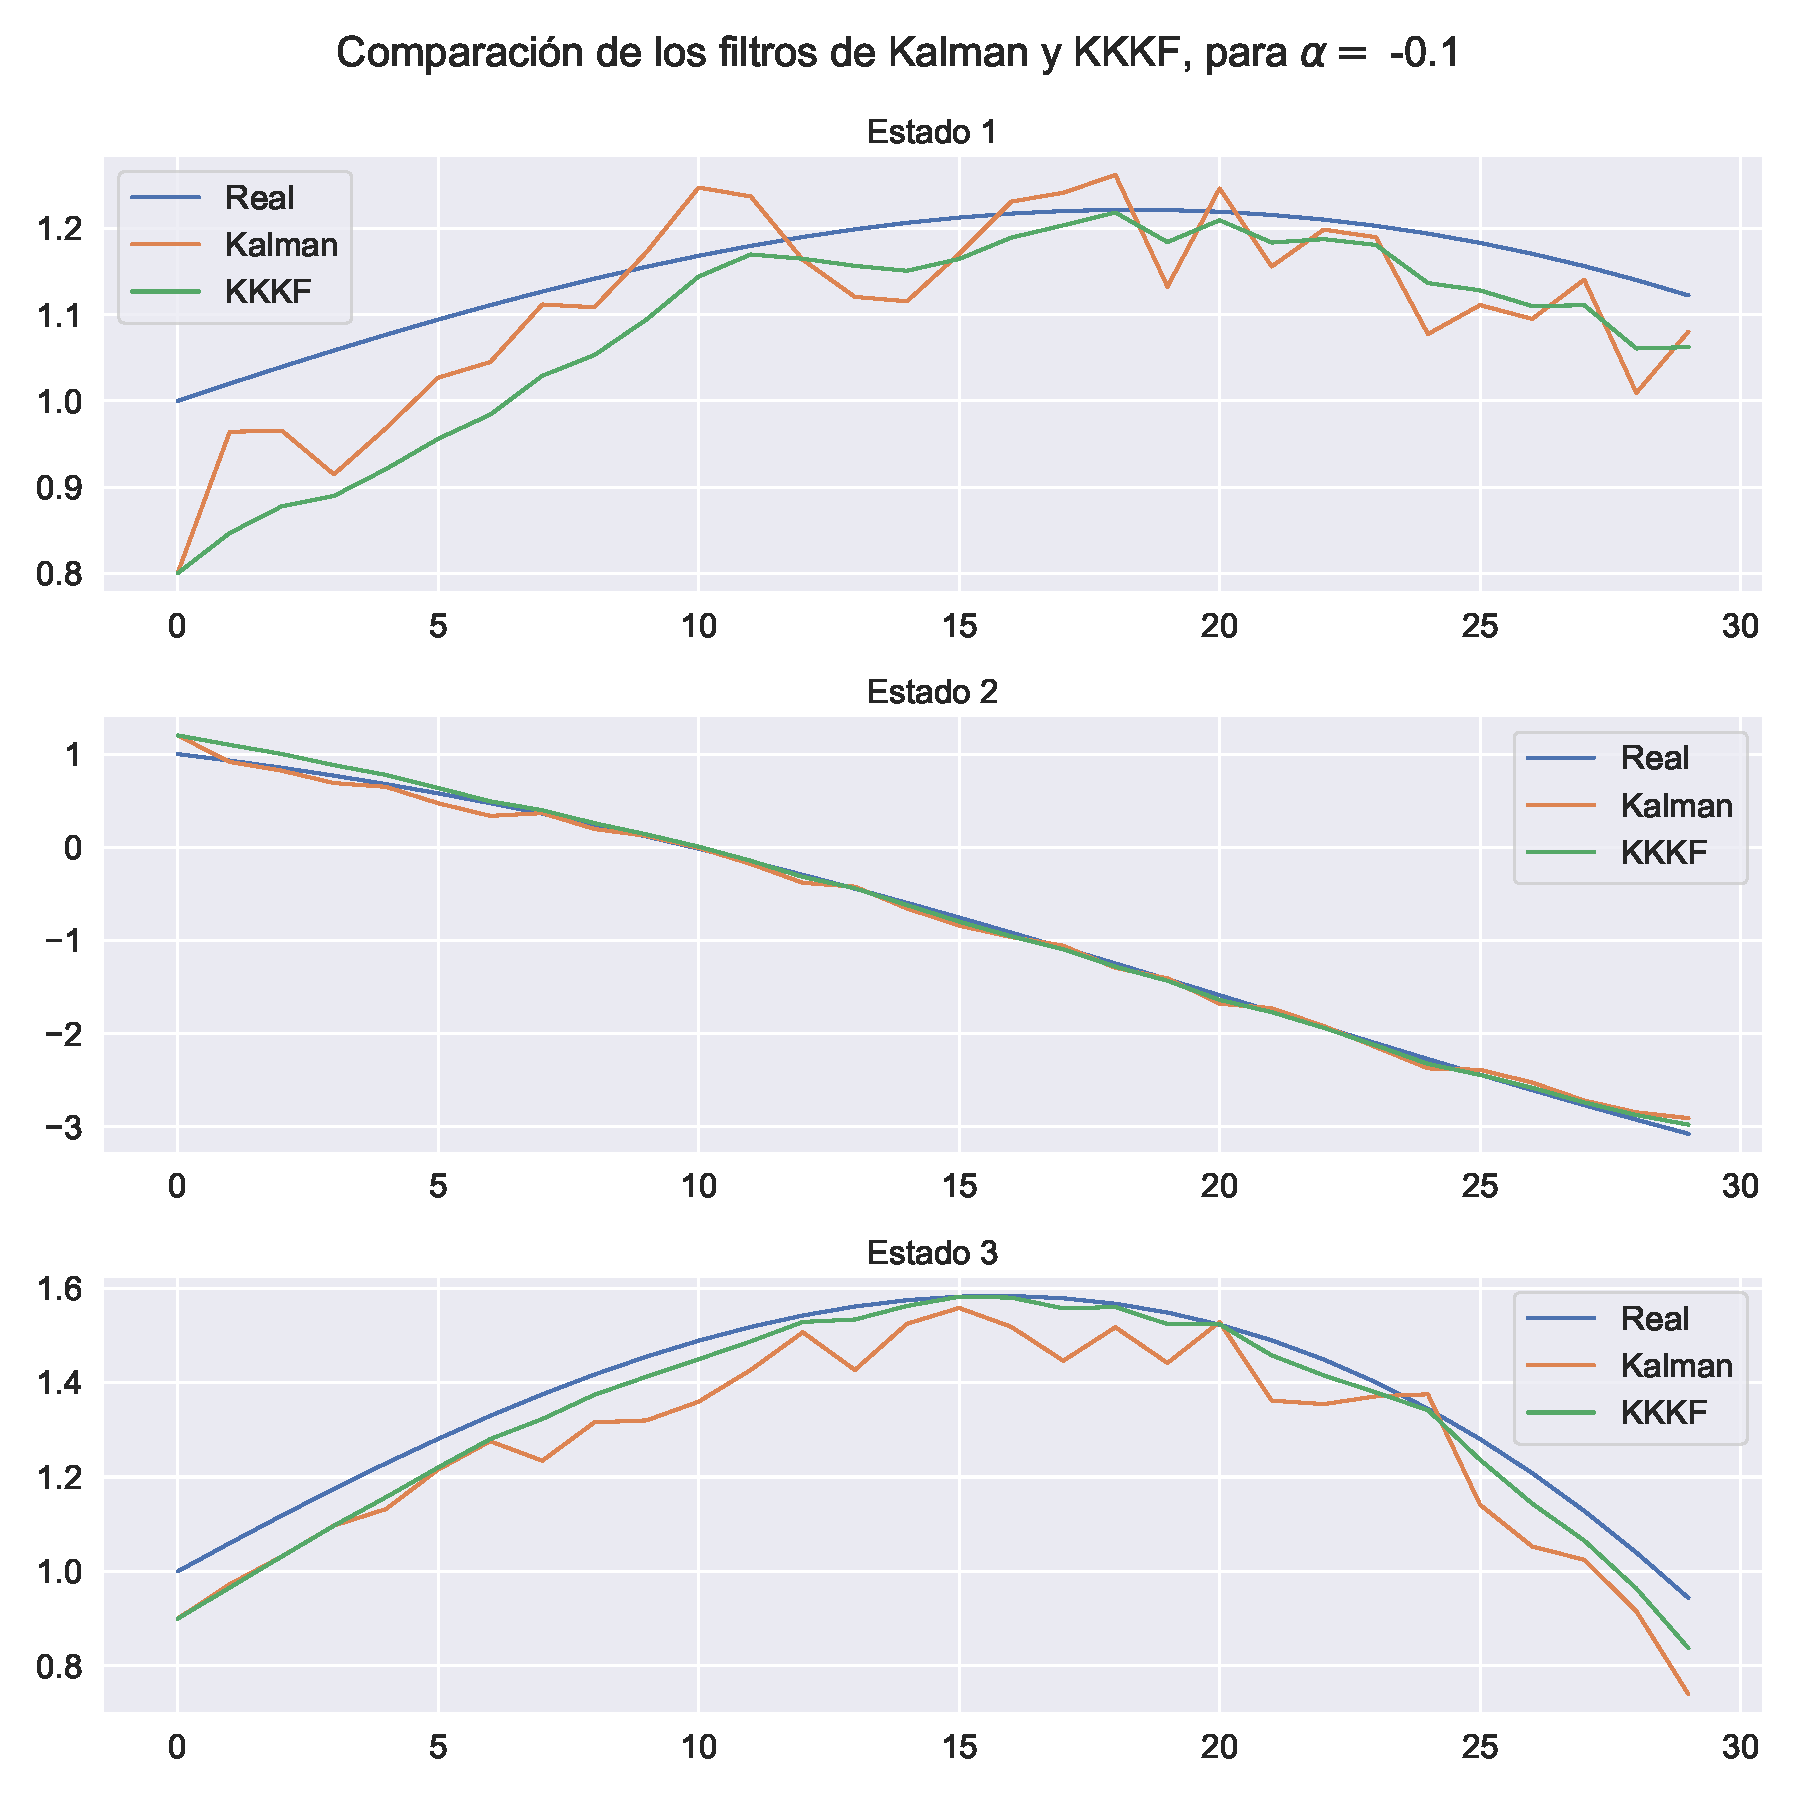
\includegraphics[width=0.9\linewidth]{img/content/chapter4/kalman_vs_kerKKF_01.pdf}
    \caption{$\alpha = -0.1$.}
    \label{fig:kalman_vs_kerKKF_01}
    \end{subfigure}
    \begin{subfigure}[b]{0.49\textwidth}
        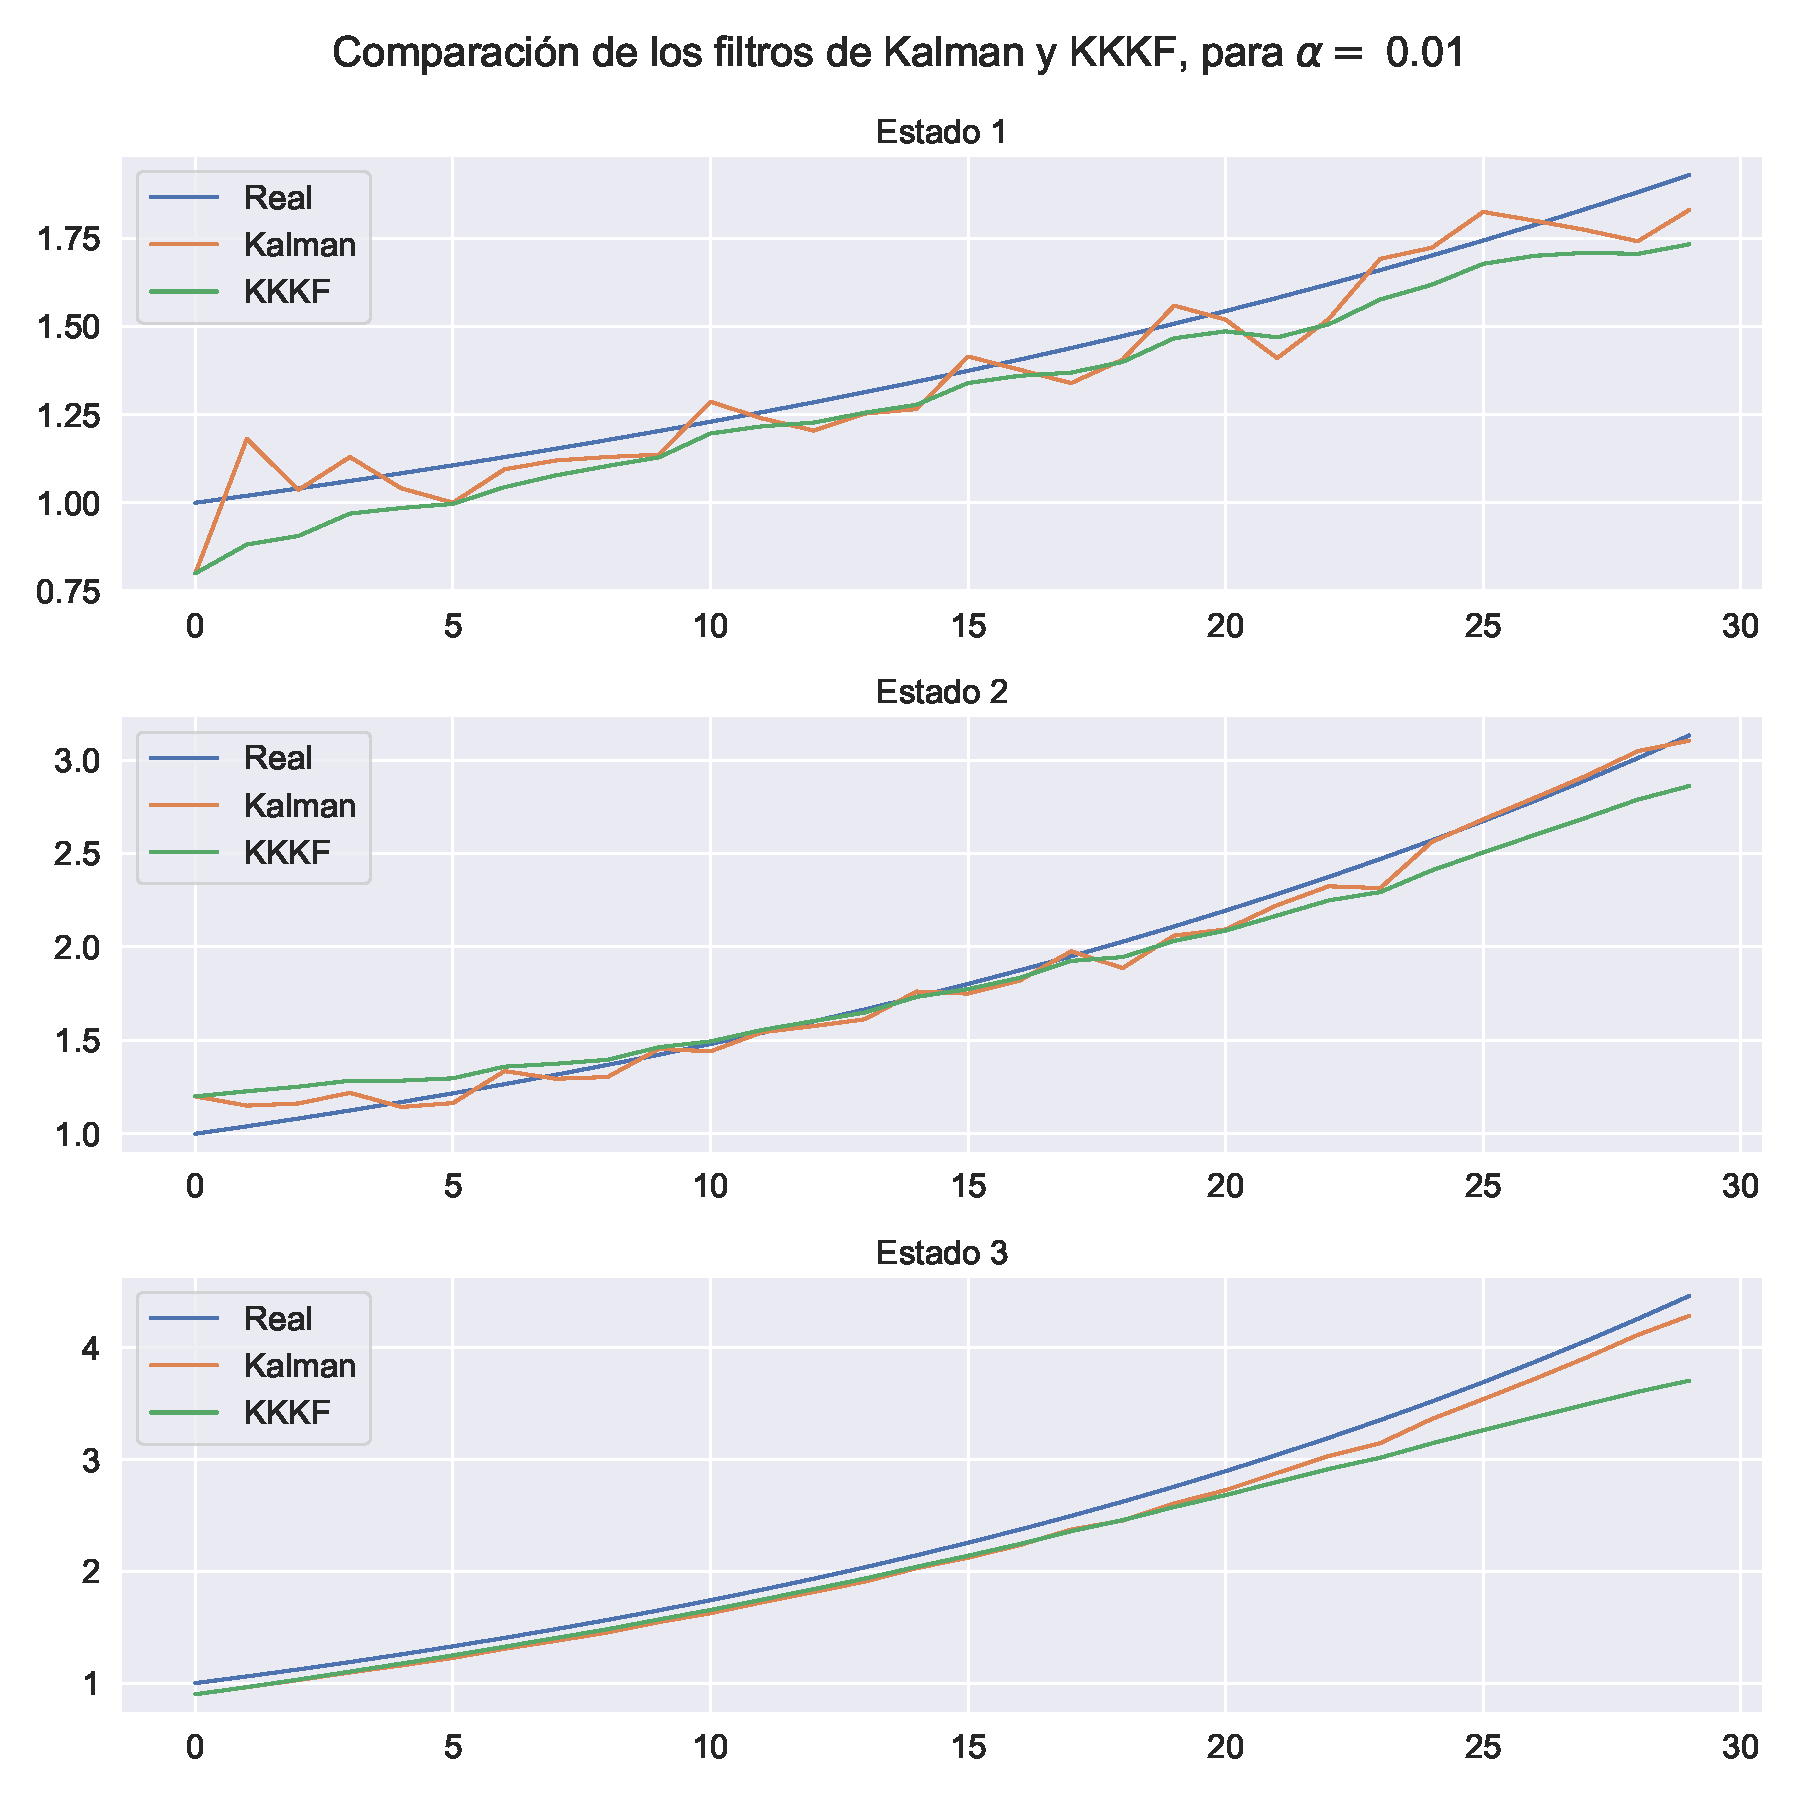
\includegraphics[width=0.9\linewidth]{img/content/chapter4/kalman_vs_kerKKF_001.pdf}
    \caption{$\alpha = 0.01$.}
    \label{fig:kalman_vs_kerKKF_001}
    \end{subfigure}
    \begin{subfigure}[b]{0.49\textwidth}
        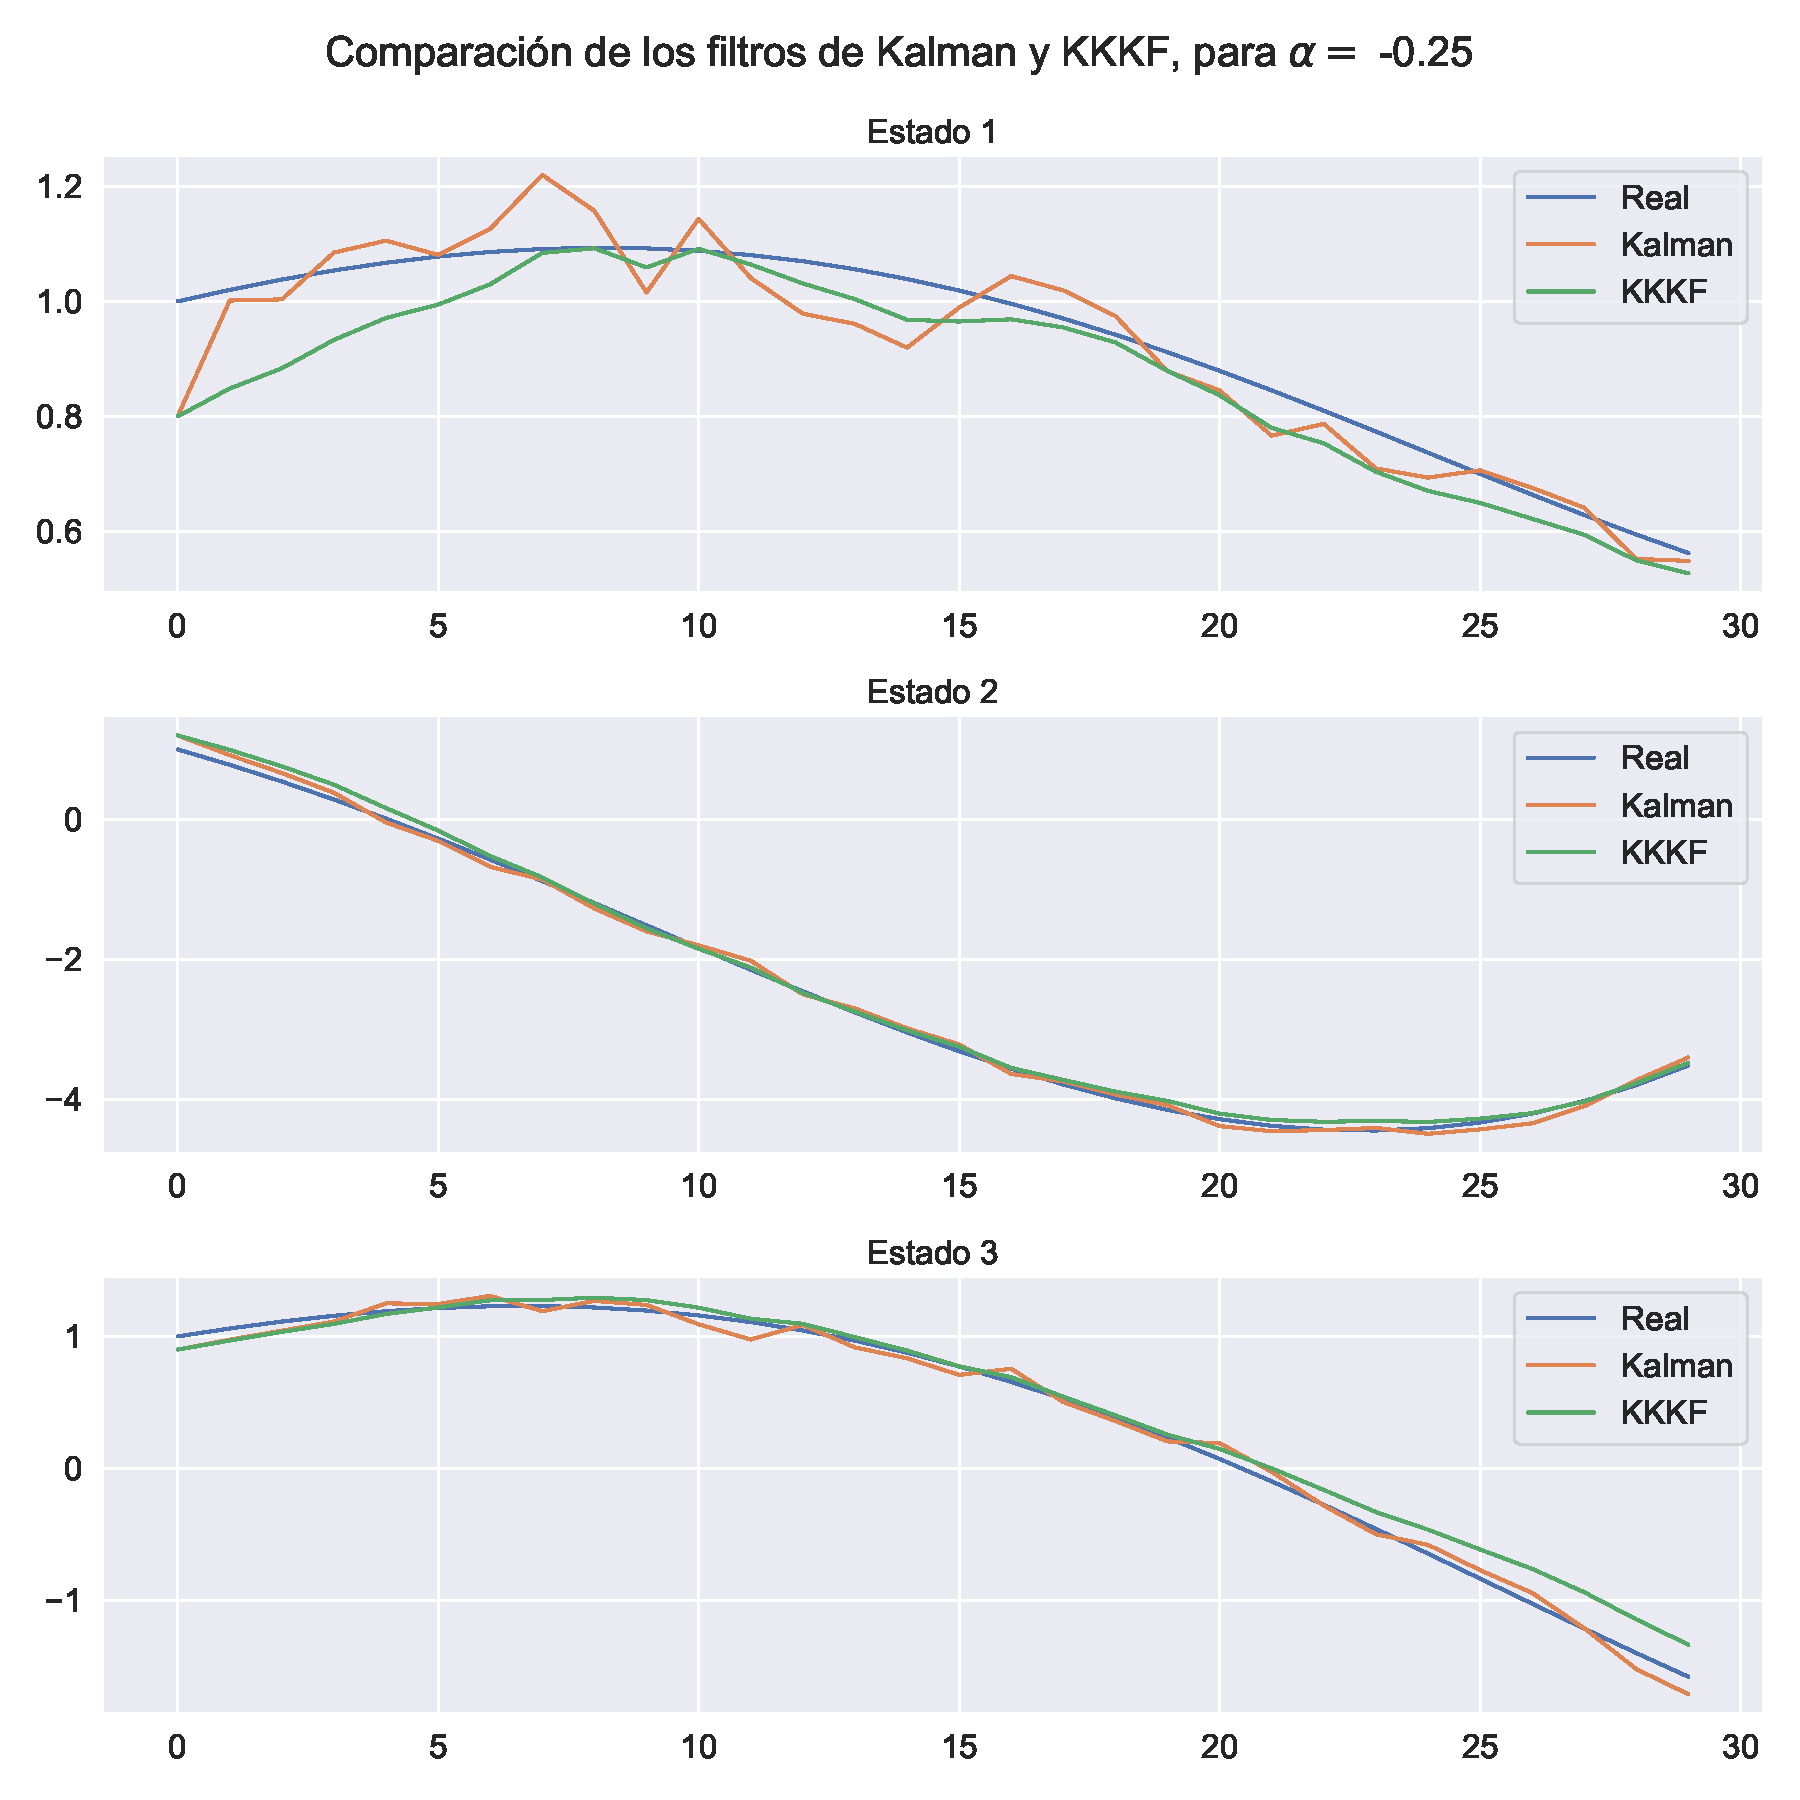
\includegraphics[width=0.9\linewidth]{img/content/chapter4/kalman_vs_kerKKF_025.pdf}
    \caption{$\alpha = -0.25$.}
    \label{fig:kalman_vs_kerKKF_025}
    \end{subfigure}
    \caption{Comparación de Kalman con kerKKF para distintos valores de $\alpha$. En línea azul se encuentra el resultado del sistema simulado sin ruidos ni de dinámica ni observación, en naranja la solución del filtro de Kalman y en verde la solución de kerKKF.}
\end{figure}

\begin{figure}[h]
    \centering
    \begin{subfigure}[b]{0.49\textwidth}
        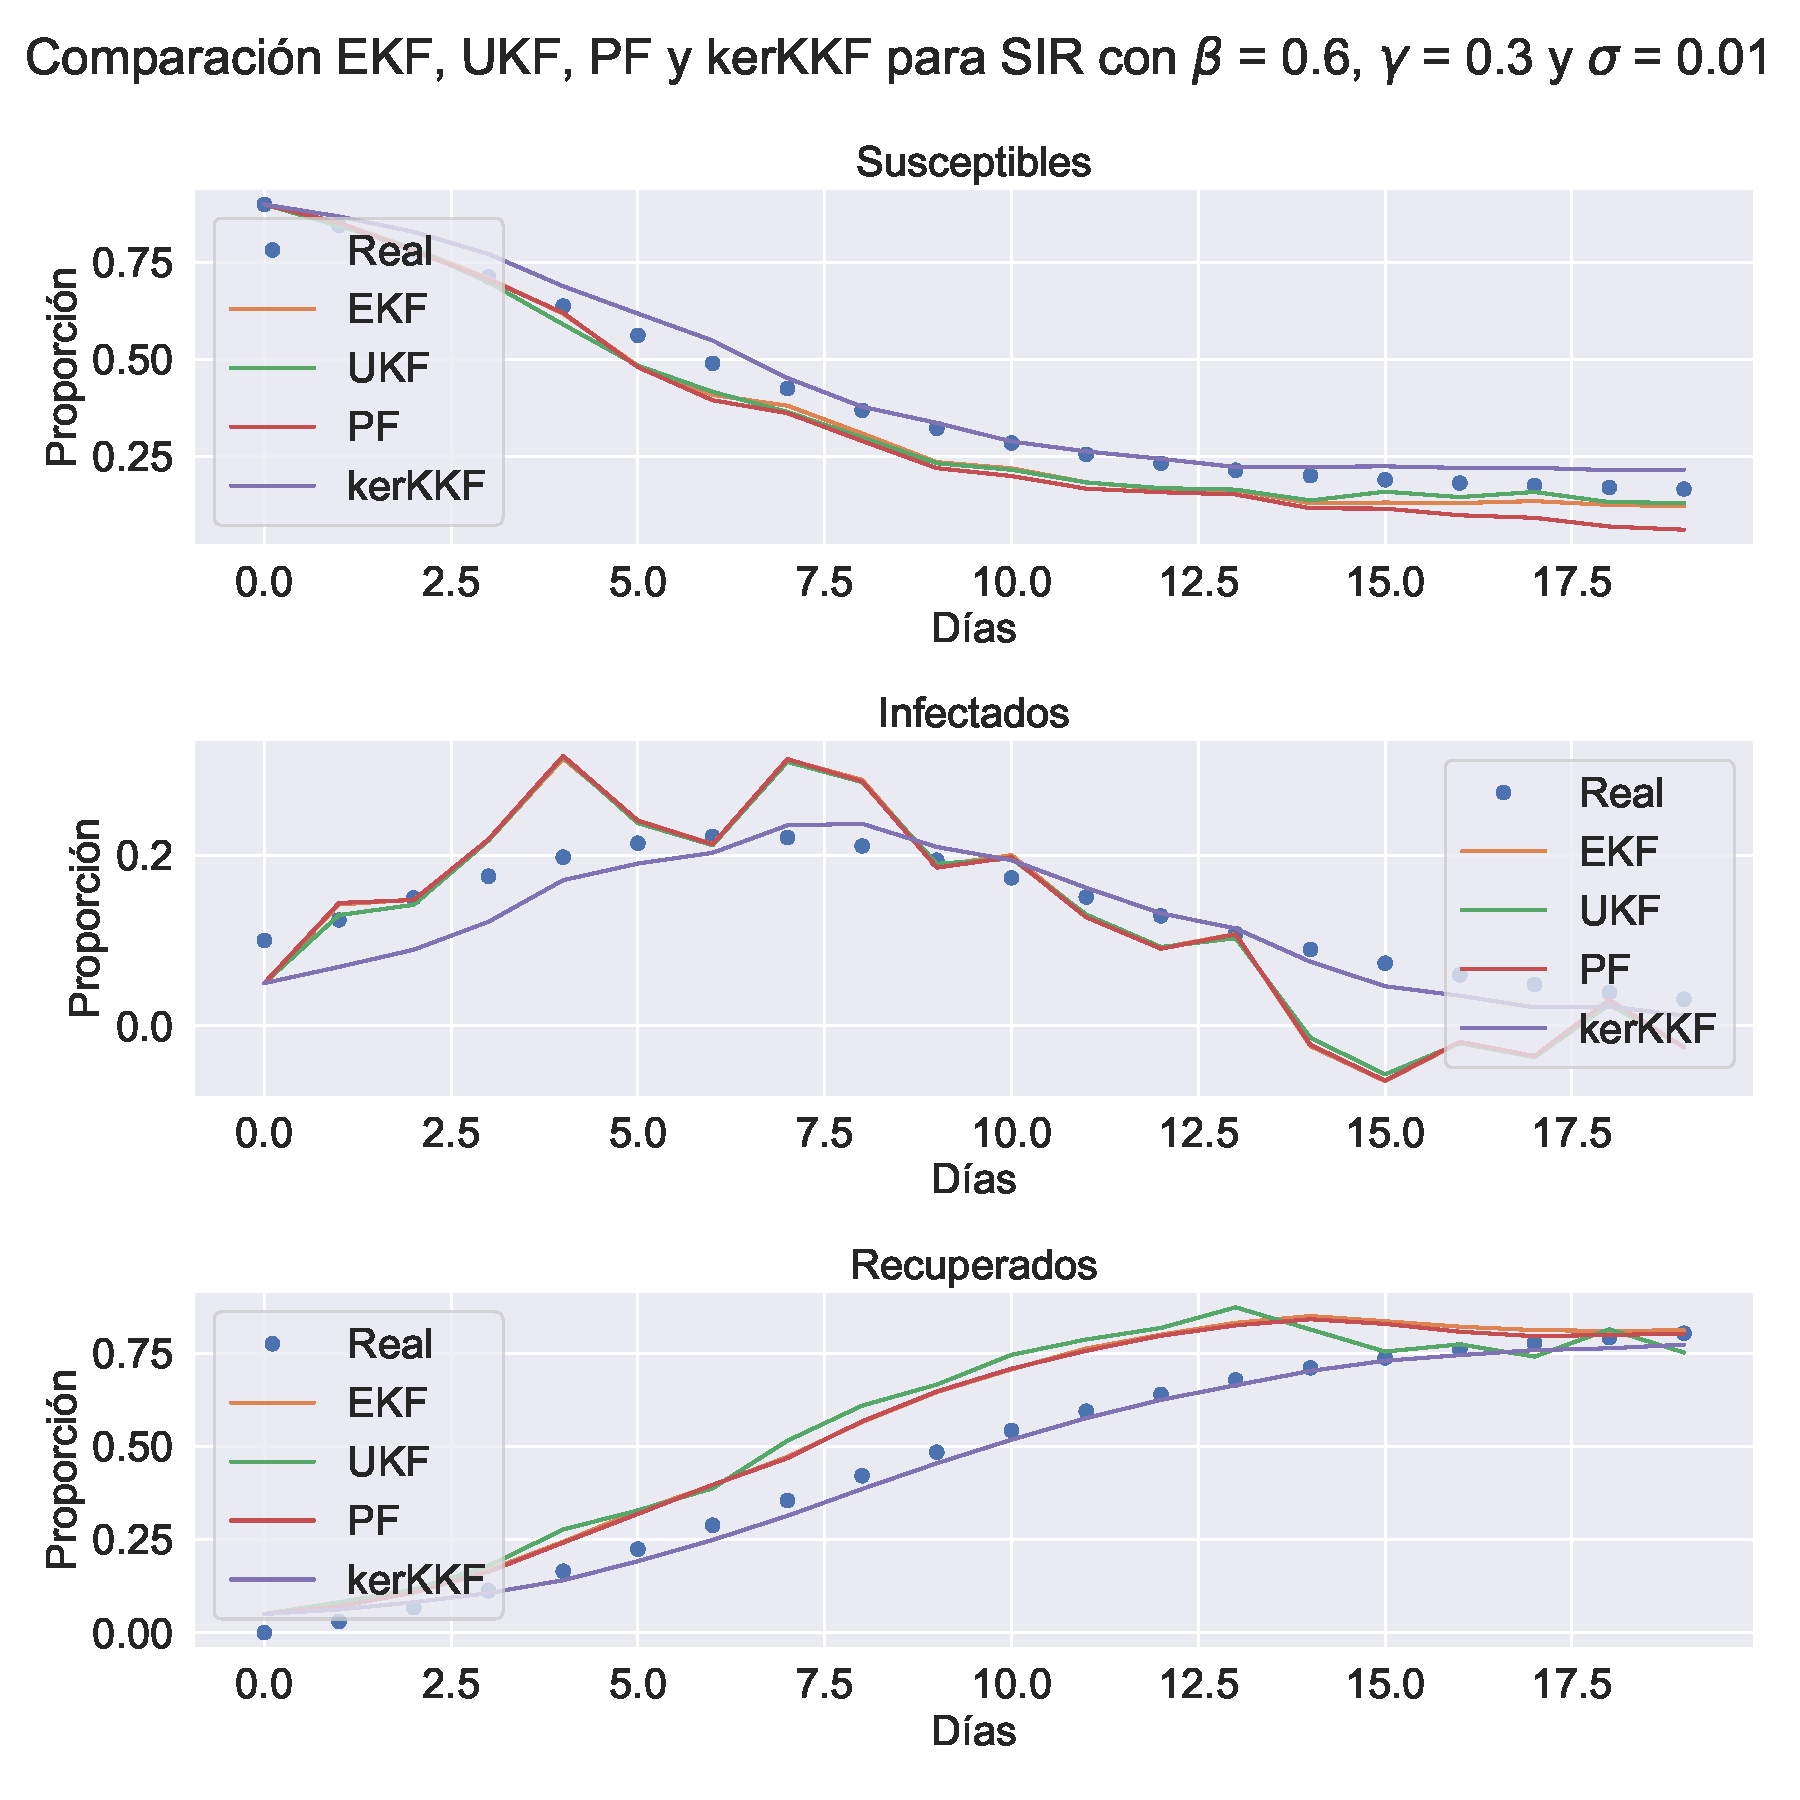
\includegraphics[width=\linewidth]{img/content/chapter4/nonlinear_filters_sir_beta_06.pdf}
    \caption{$\beta = 0.6$.}
    \label{fig:nonlinear_filters_sir_beta_06}
    \end{subfigure}
    \begin{subfigure}[b]{0.49\textwidth}
        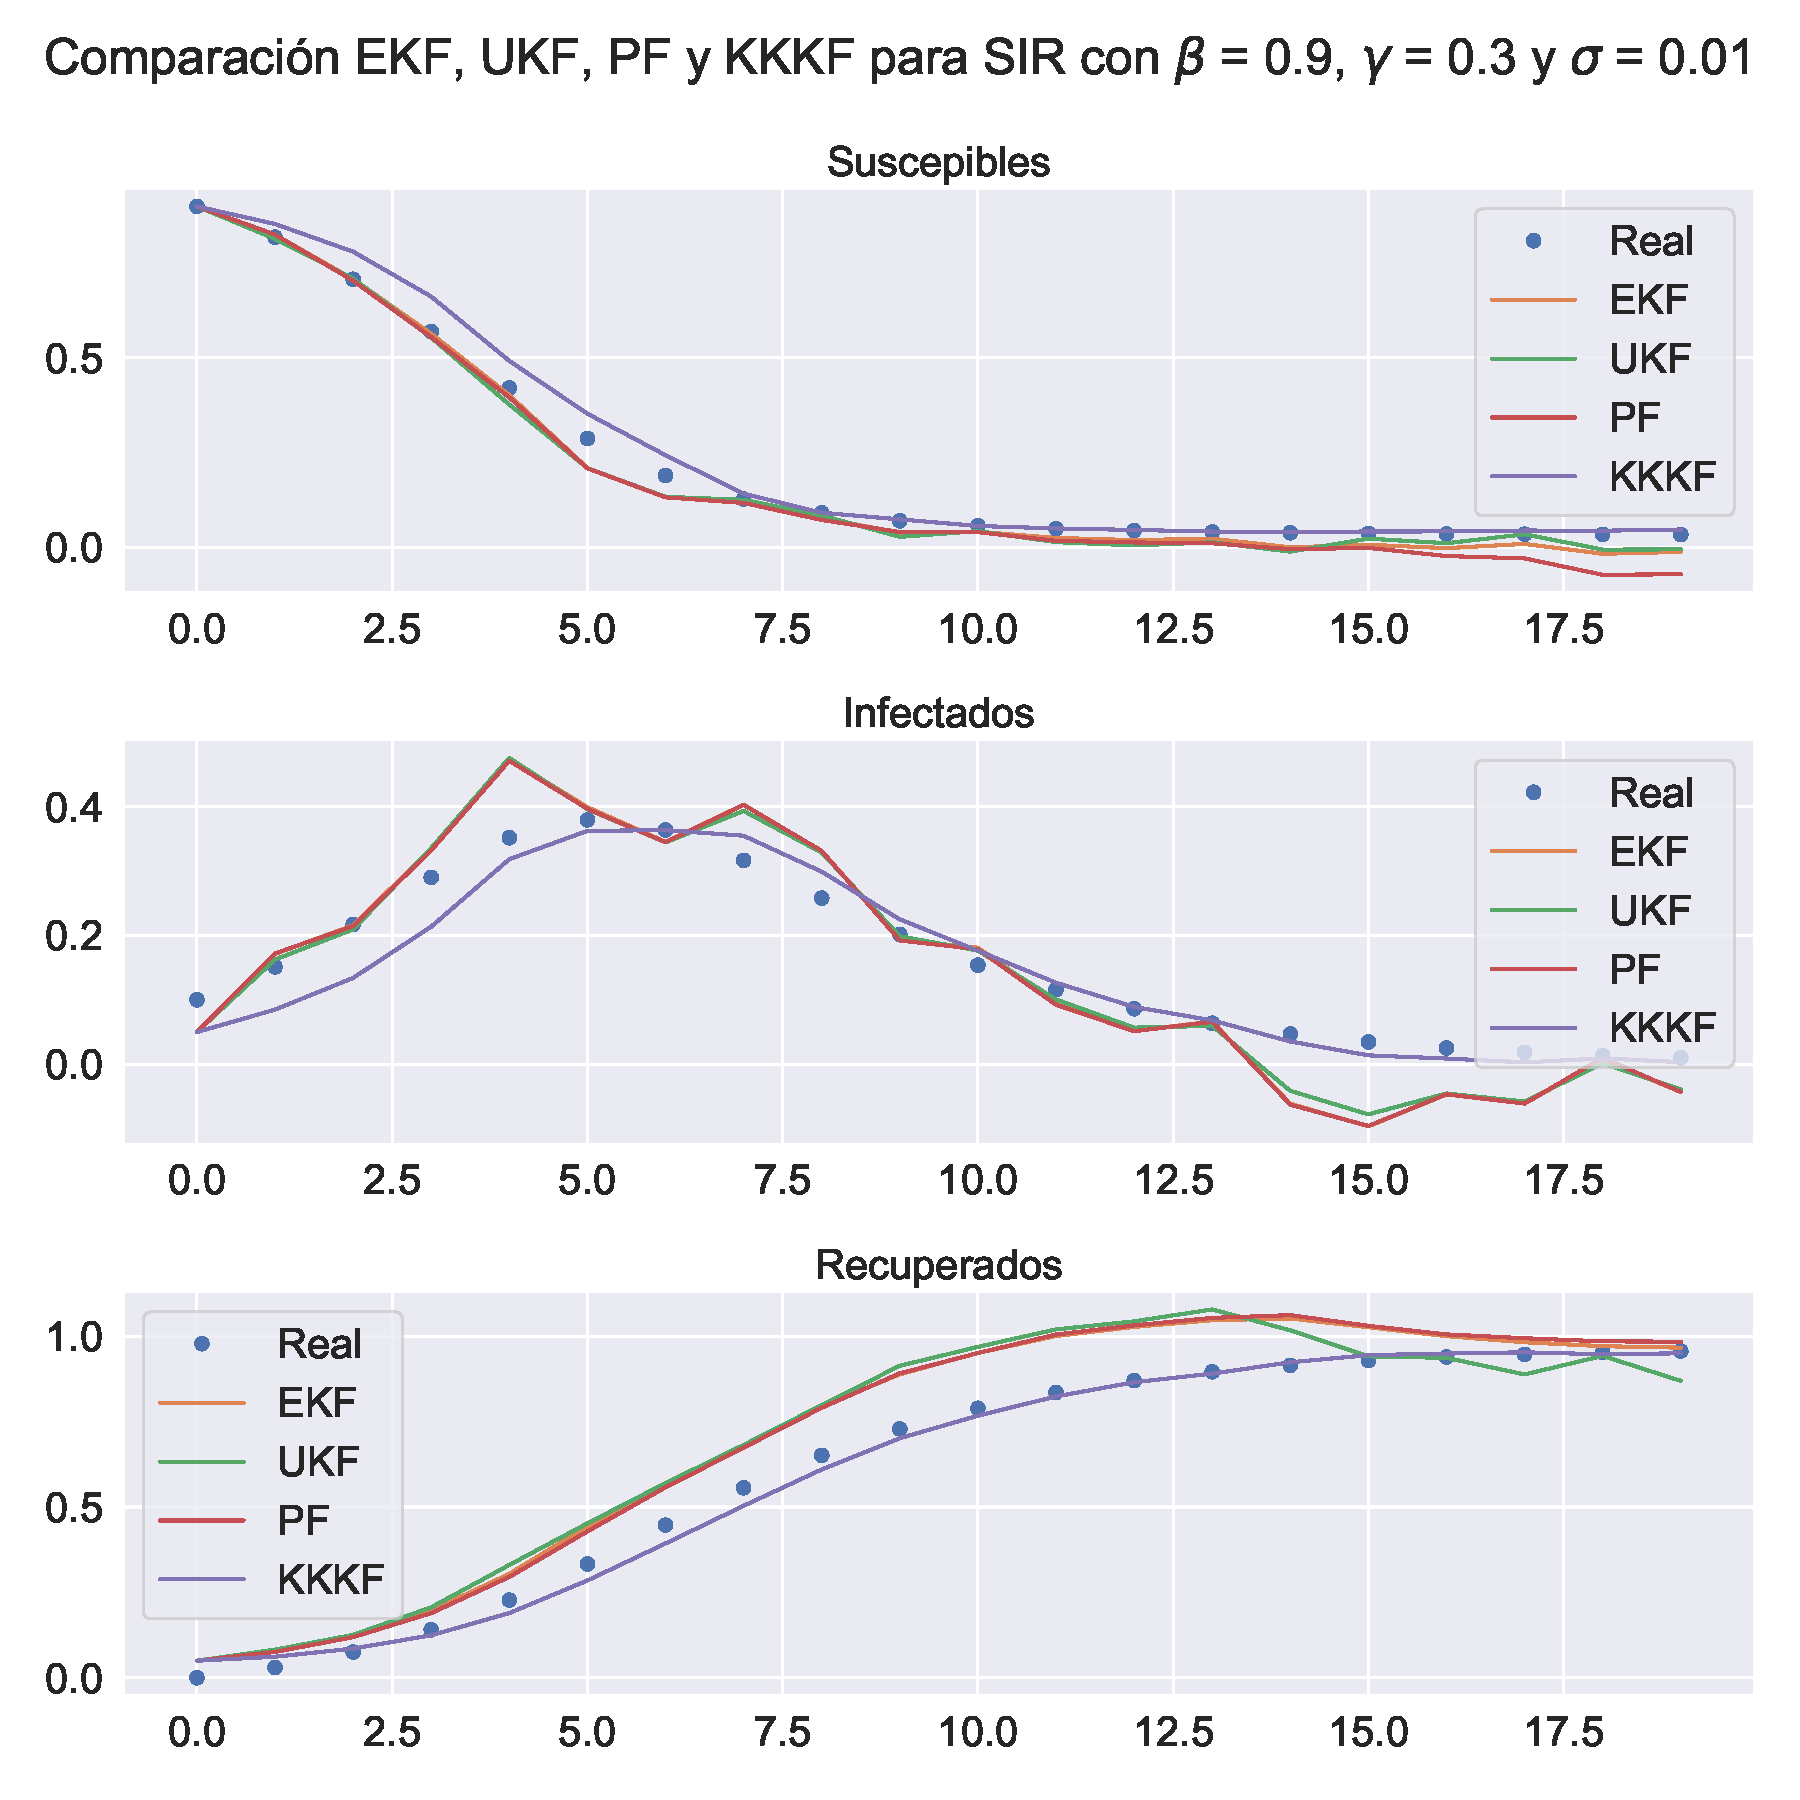
\includegraphics[width=\linewidth]{img/content/chapter4/nonlinear_filters_sir_beta_09.pdf}
    \caption{$\beta = 0.9$.}
    \label{fig:nonlinear_filters_sir_beta_09}
    \end{subfigure}
    \begin{subfigure}[b]{0.49\textwidth}
        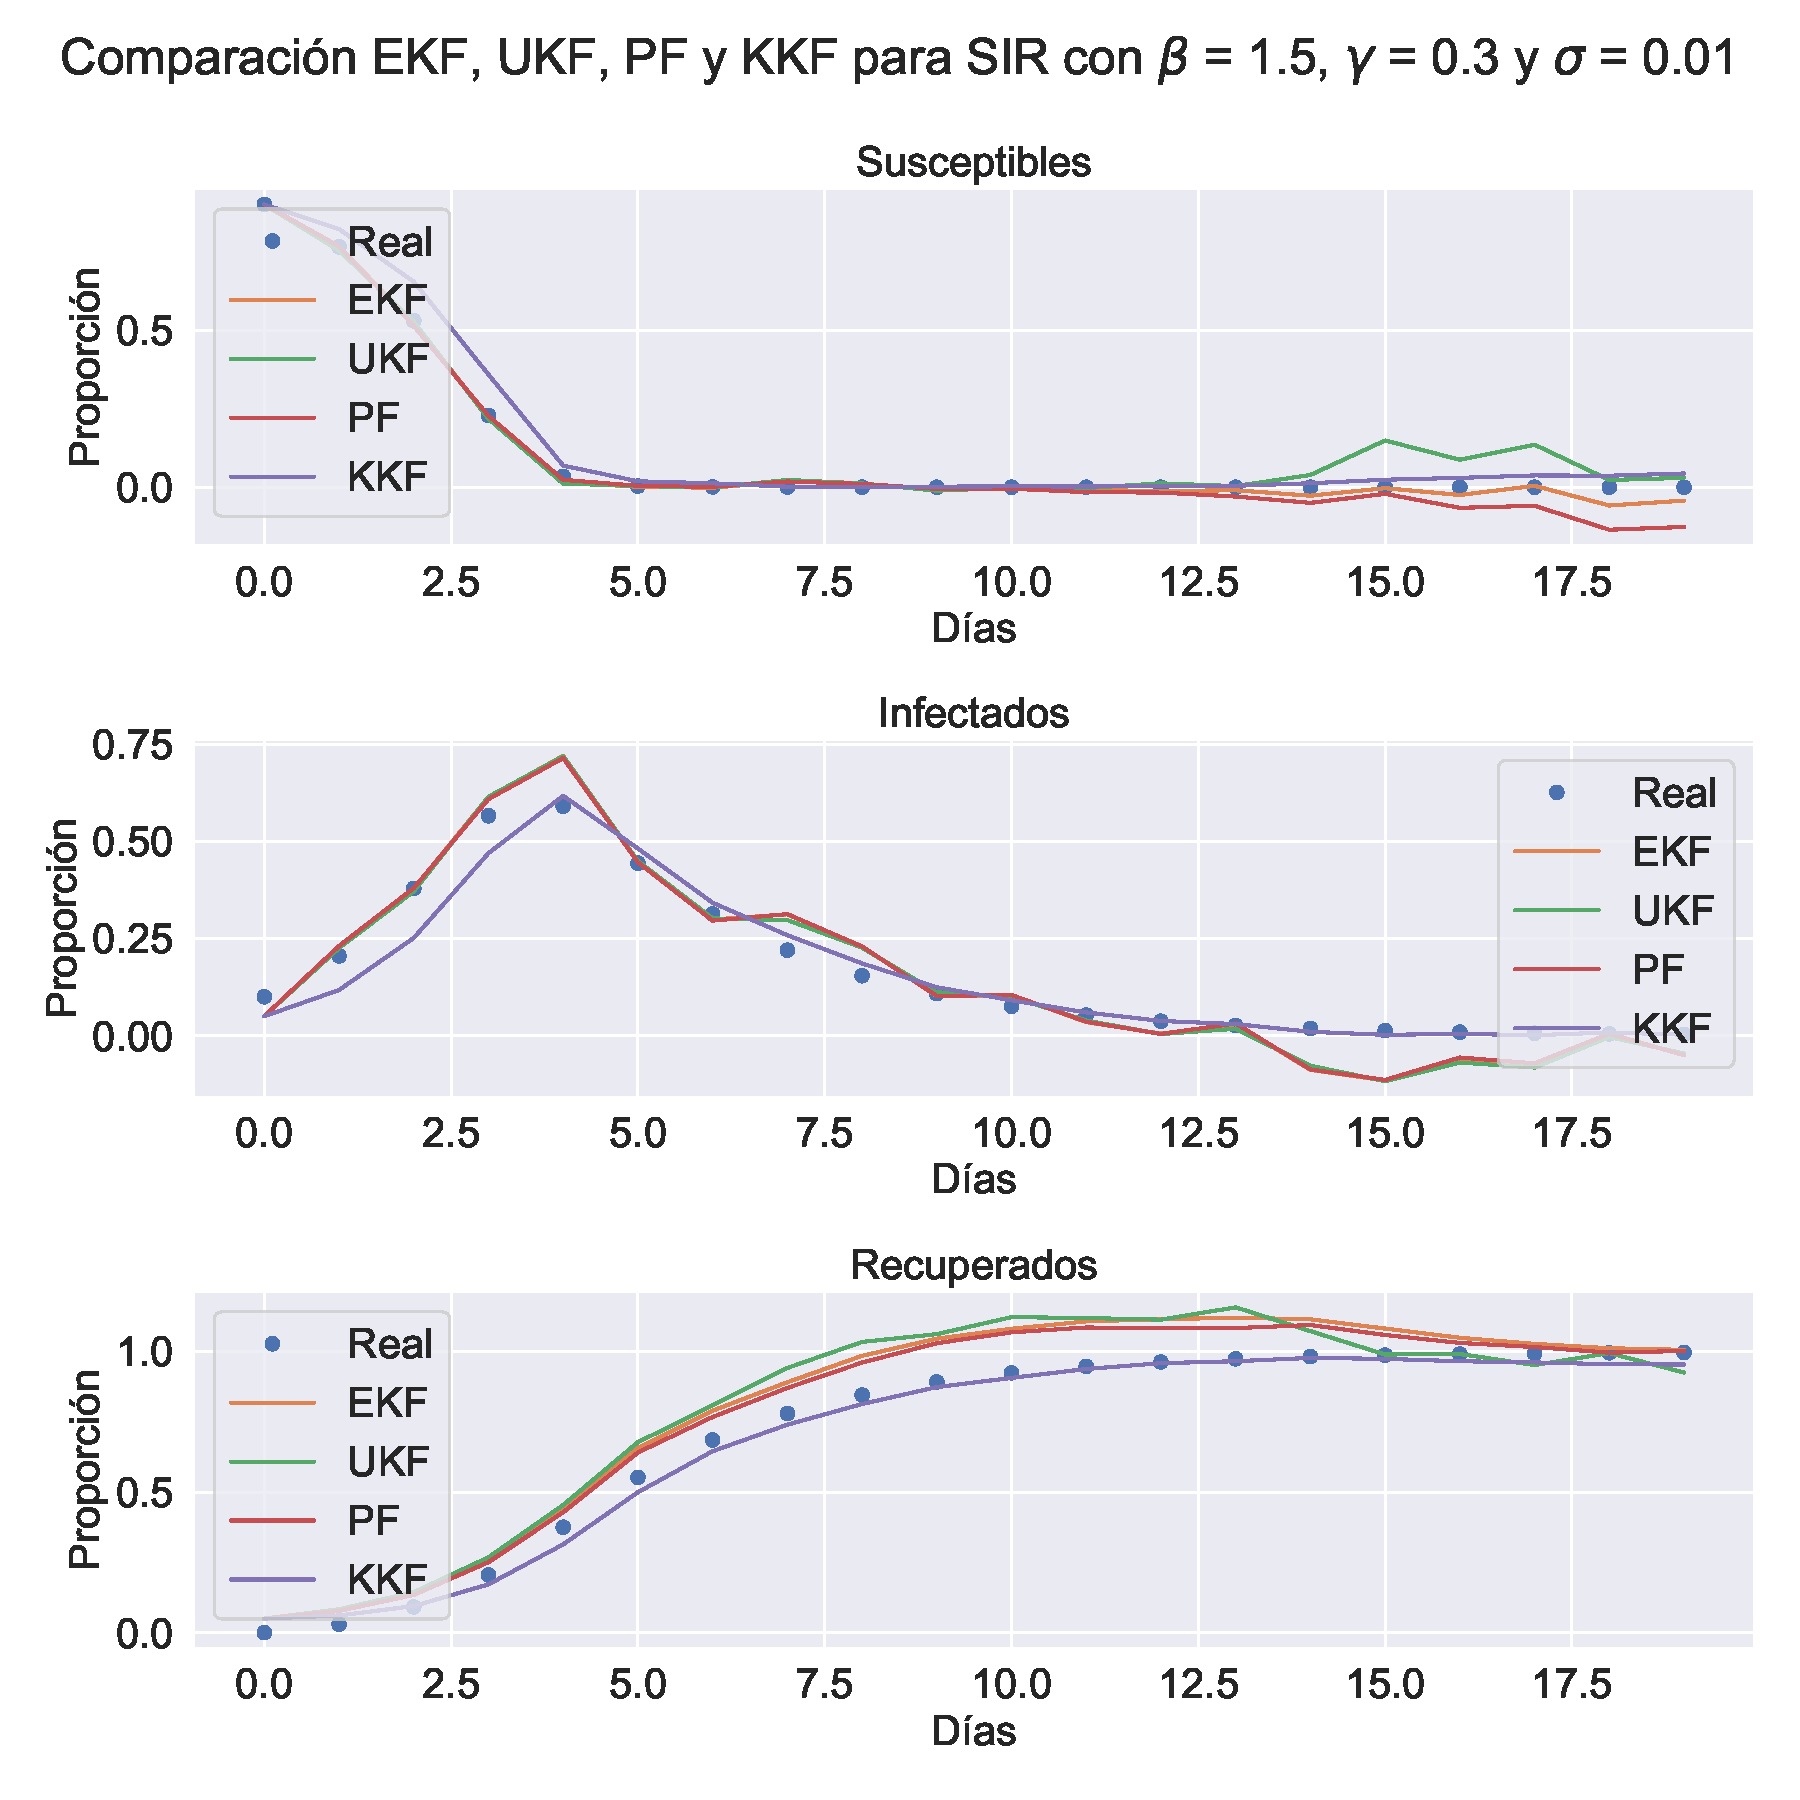
\includegraphics[width=\linewidth]{img/content/chapter4/nonlinear_filters_sir_beta_15.pdf}
    \caption{$\beta = 1.5$.}
    \label{fig:nonlinear_filters_sir_beta_15}
    \end{subfigure}
    \caption{Comparación de resultados de las trayectorias generadas por los filtros EKF (naranja), UKF (verde), PF (rojo) y kerKKF (púrpura), junto con la trayectoria real (puntos azules) sin ruidos, ni de dinámica ni de observación, esto para cada uno de los estados del modelo SIR. $\beta$ varía en cada caso para (a), (b) y (c), mientras que $\gamma = 0.3$ y $\sigma = 0.01$ fijos.}
\end{figure}

\begin{table}[h]
    \caption{Errores para distintos valores de $\beta$, parámetro que representa la no linealidad del sistema. Esto para $\gamma = 0.3$ y $\sigma = 0.01$ fijos.}
    \begin{subtable}{\linewidth}
        \centering
    \caption{Errores para $\beta = 0.6$ y $\gamma = 0.3$}
    \begin{tabular}{|c|c|c|c|c|}
    \hline
    \textbf{Estado} & \textbf{EKF} & \textbf{UKF} & \textbf{PF} & \textbf{kerKKF} \\ \hline
    S & 0.2442 & 0.2379 & 0.3305 & 0.1629 \\ \hline
    I & 0.2904 & 0.2815 & 0.2903 & 0.1352 \\ \hline
    R & 0.4874 & 0.5503 & 0.4732 & 0.1210 \\ \hline
    \end{tabular}
    \label{tab:errores_beta_gamma_06}
    \end{subtable}
    \begin{subtable}{\linewidth}
        \centering
    \caption{Errores para $\beta = 0.9$ y $\gamma = 0.3$}
    \begin{tabular}{|c|c|c|c|c|}
    \hline
    \textbf{Estado} & \textbf{EKF} & \textbf{UKF} & \textbf{PF} & \textbf{kerKKF} \\ \hline
    S & 0.1486 & 0.1533 & 0.2195 & 0.1672 \\ \hline
    I & 0.2808 & 0.2590 & 0.2798 & 0.1628 \\ \hline
    R & 0.4866 & 0.5246 & 0.4907 & 0.1300 \\ \hline
    \end{tabular}
    \label{tab:errores_beta_gamma_09}
    \end{subtable}
    \begin{subtable}{\linewidth}
        \centering
    \caption{Errores para $\beta = 1.5$ y $\gamma = 0.3$}
    \begin{tabular}{|c|c|c|c|c|}
    \hline
    \textbf{Estado} & \textbf{EKF} & \textbf{UKF} & \textbf{PF} & \textbf{kerKKF} \\ \hline
    S & 0.0885 & 0.2296 & 0.2292 & 0.1906 \\ \hline
    I & 0.2834 & 0.2788 & 0.2816 & 0.1934 \\ \hline
    R & 0.4671 & 0.5295 & 0.4042 & 0.1435 \\ \hline
    \end{tabular}
    \label{tab:errores_beta_gamma_15}
    \end{subtable}
\end{table}

\begin{figure}[h]
    \centering
    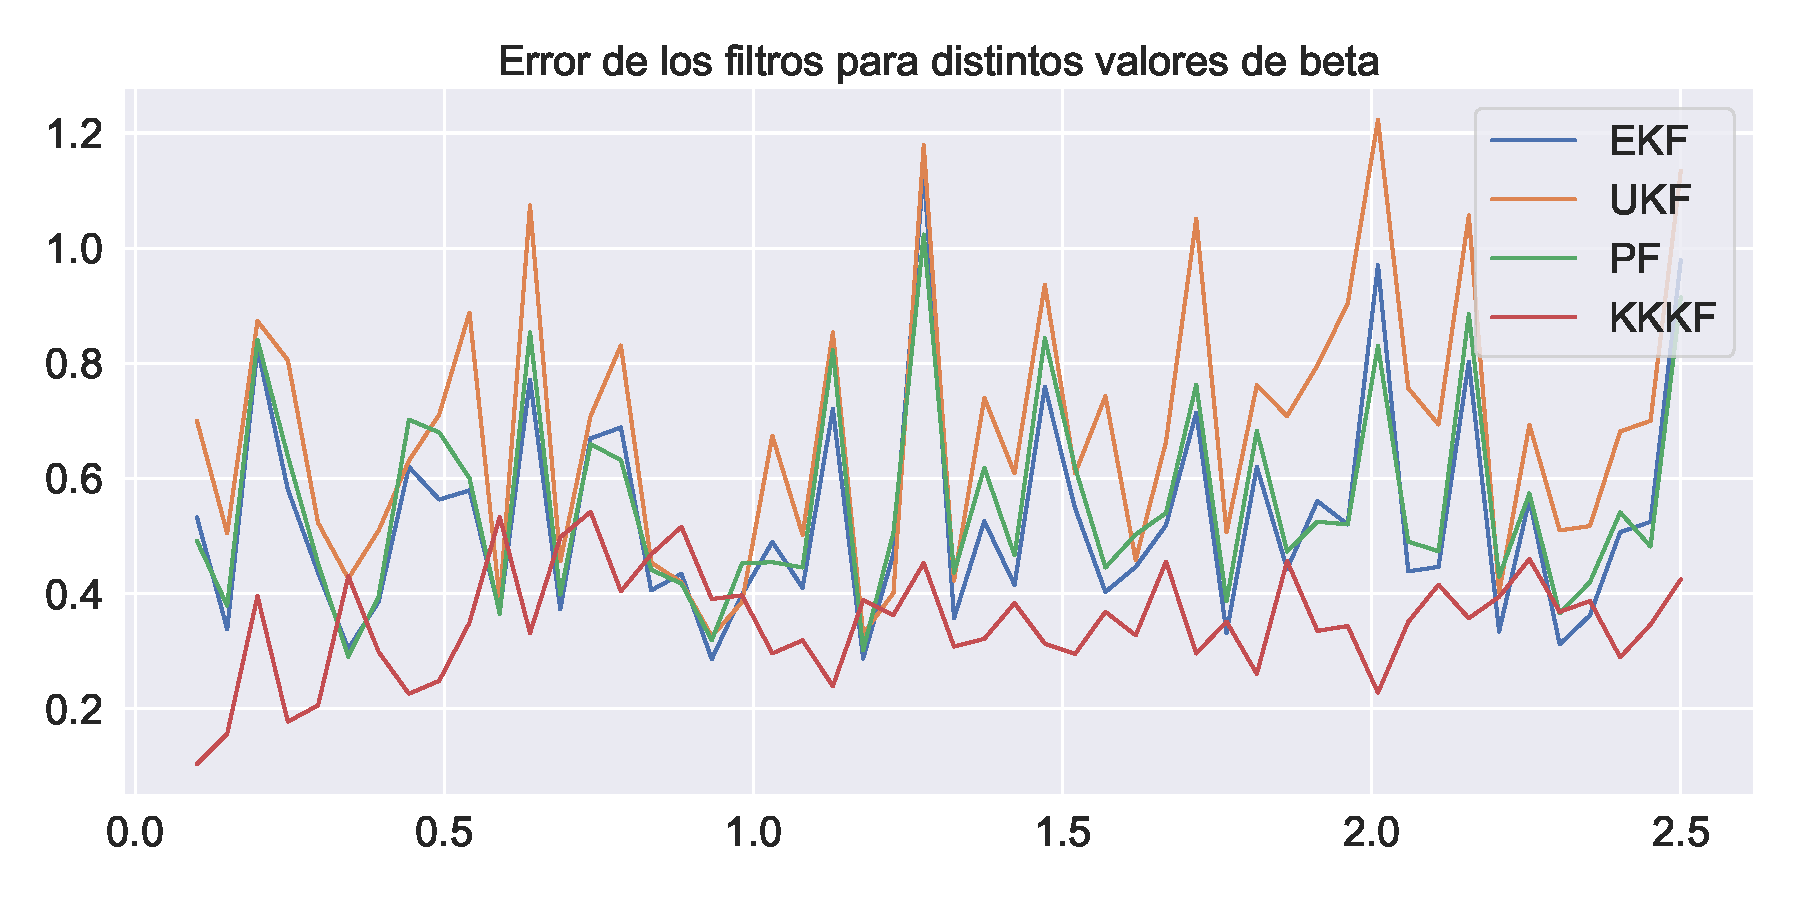
\includegraphics[width=0.8\linewidth]{img/content/chapter4/nonlinear_filters_sir_error_beta.pdf}
    \caption{Error en norma de EKF (azul), UKF (naranja), PF (verde) y kerKKF (rojo) para distintos valores de $\beta$ entre $0.1$ y $2.5$.}
    \label{fig:nonlinear_filters_sir_error_beta}
\end{figure}

\begin{figure}[h]
    \centering
    \begin{subfigure}[b]{0.49\textwidth}
    \centering
         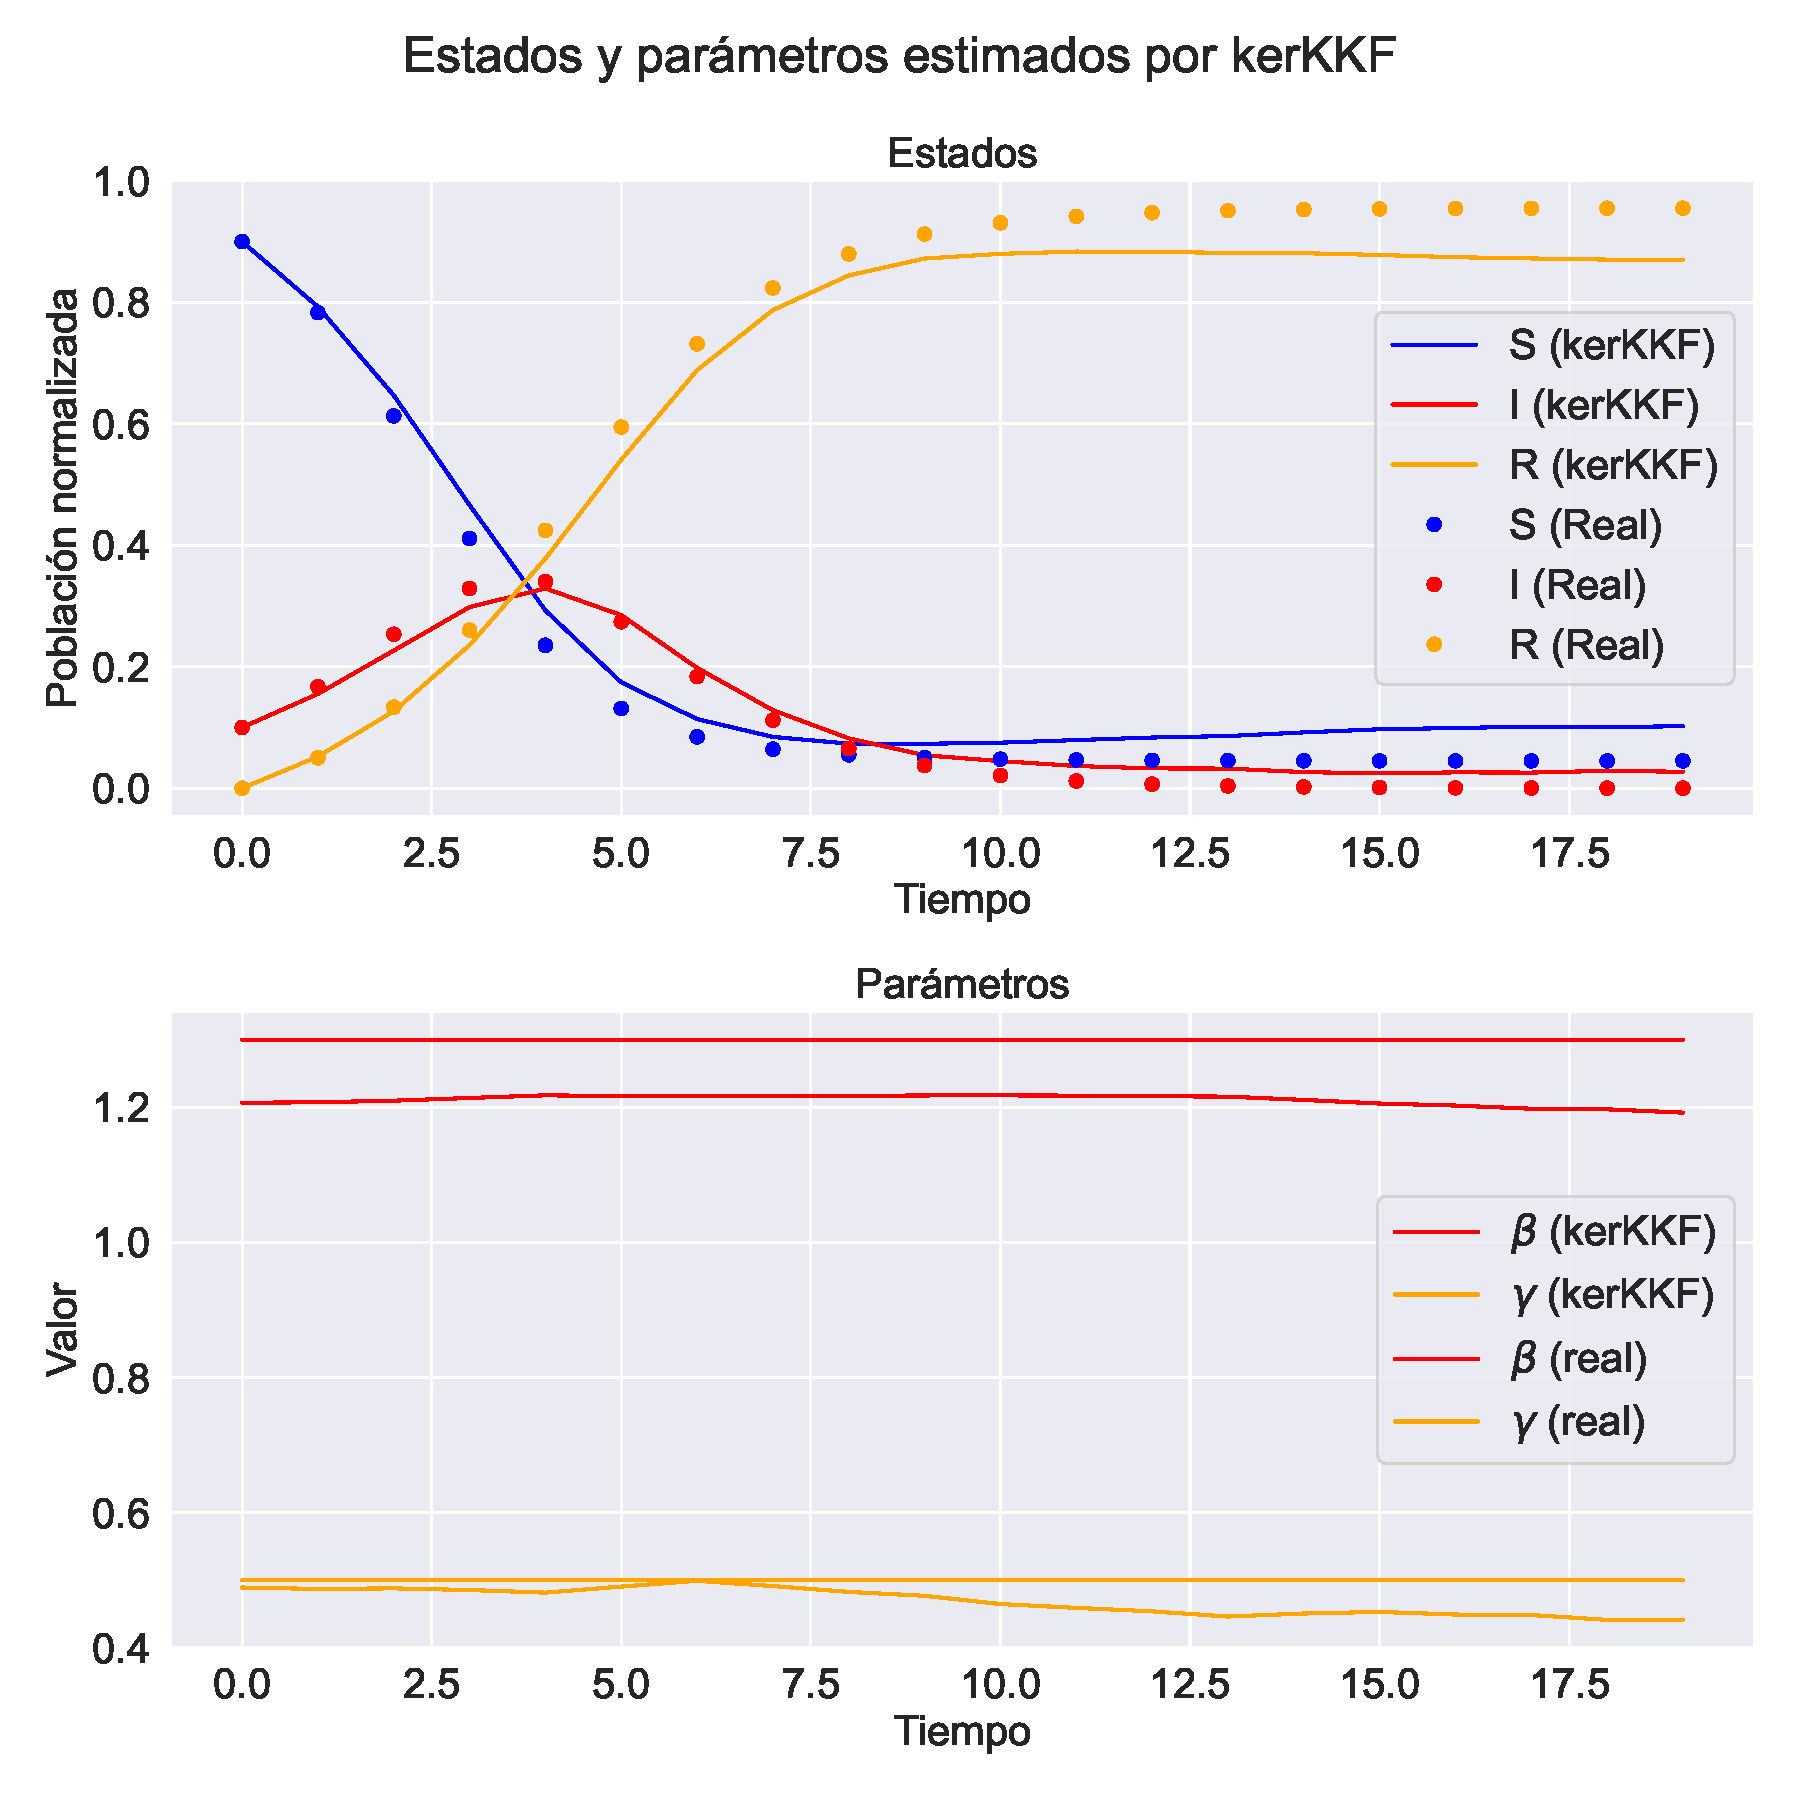
\includegraphics[width=\linewidth]{img/content/chapter4/nonlinear_filters_sir_params.pdf}
    \caption{}
    \end{subfigure}
   \begin{subfigure}[b]{0.49\textwidth}
   \centering
       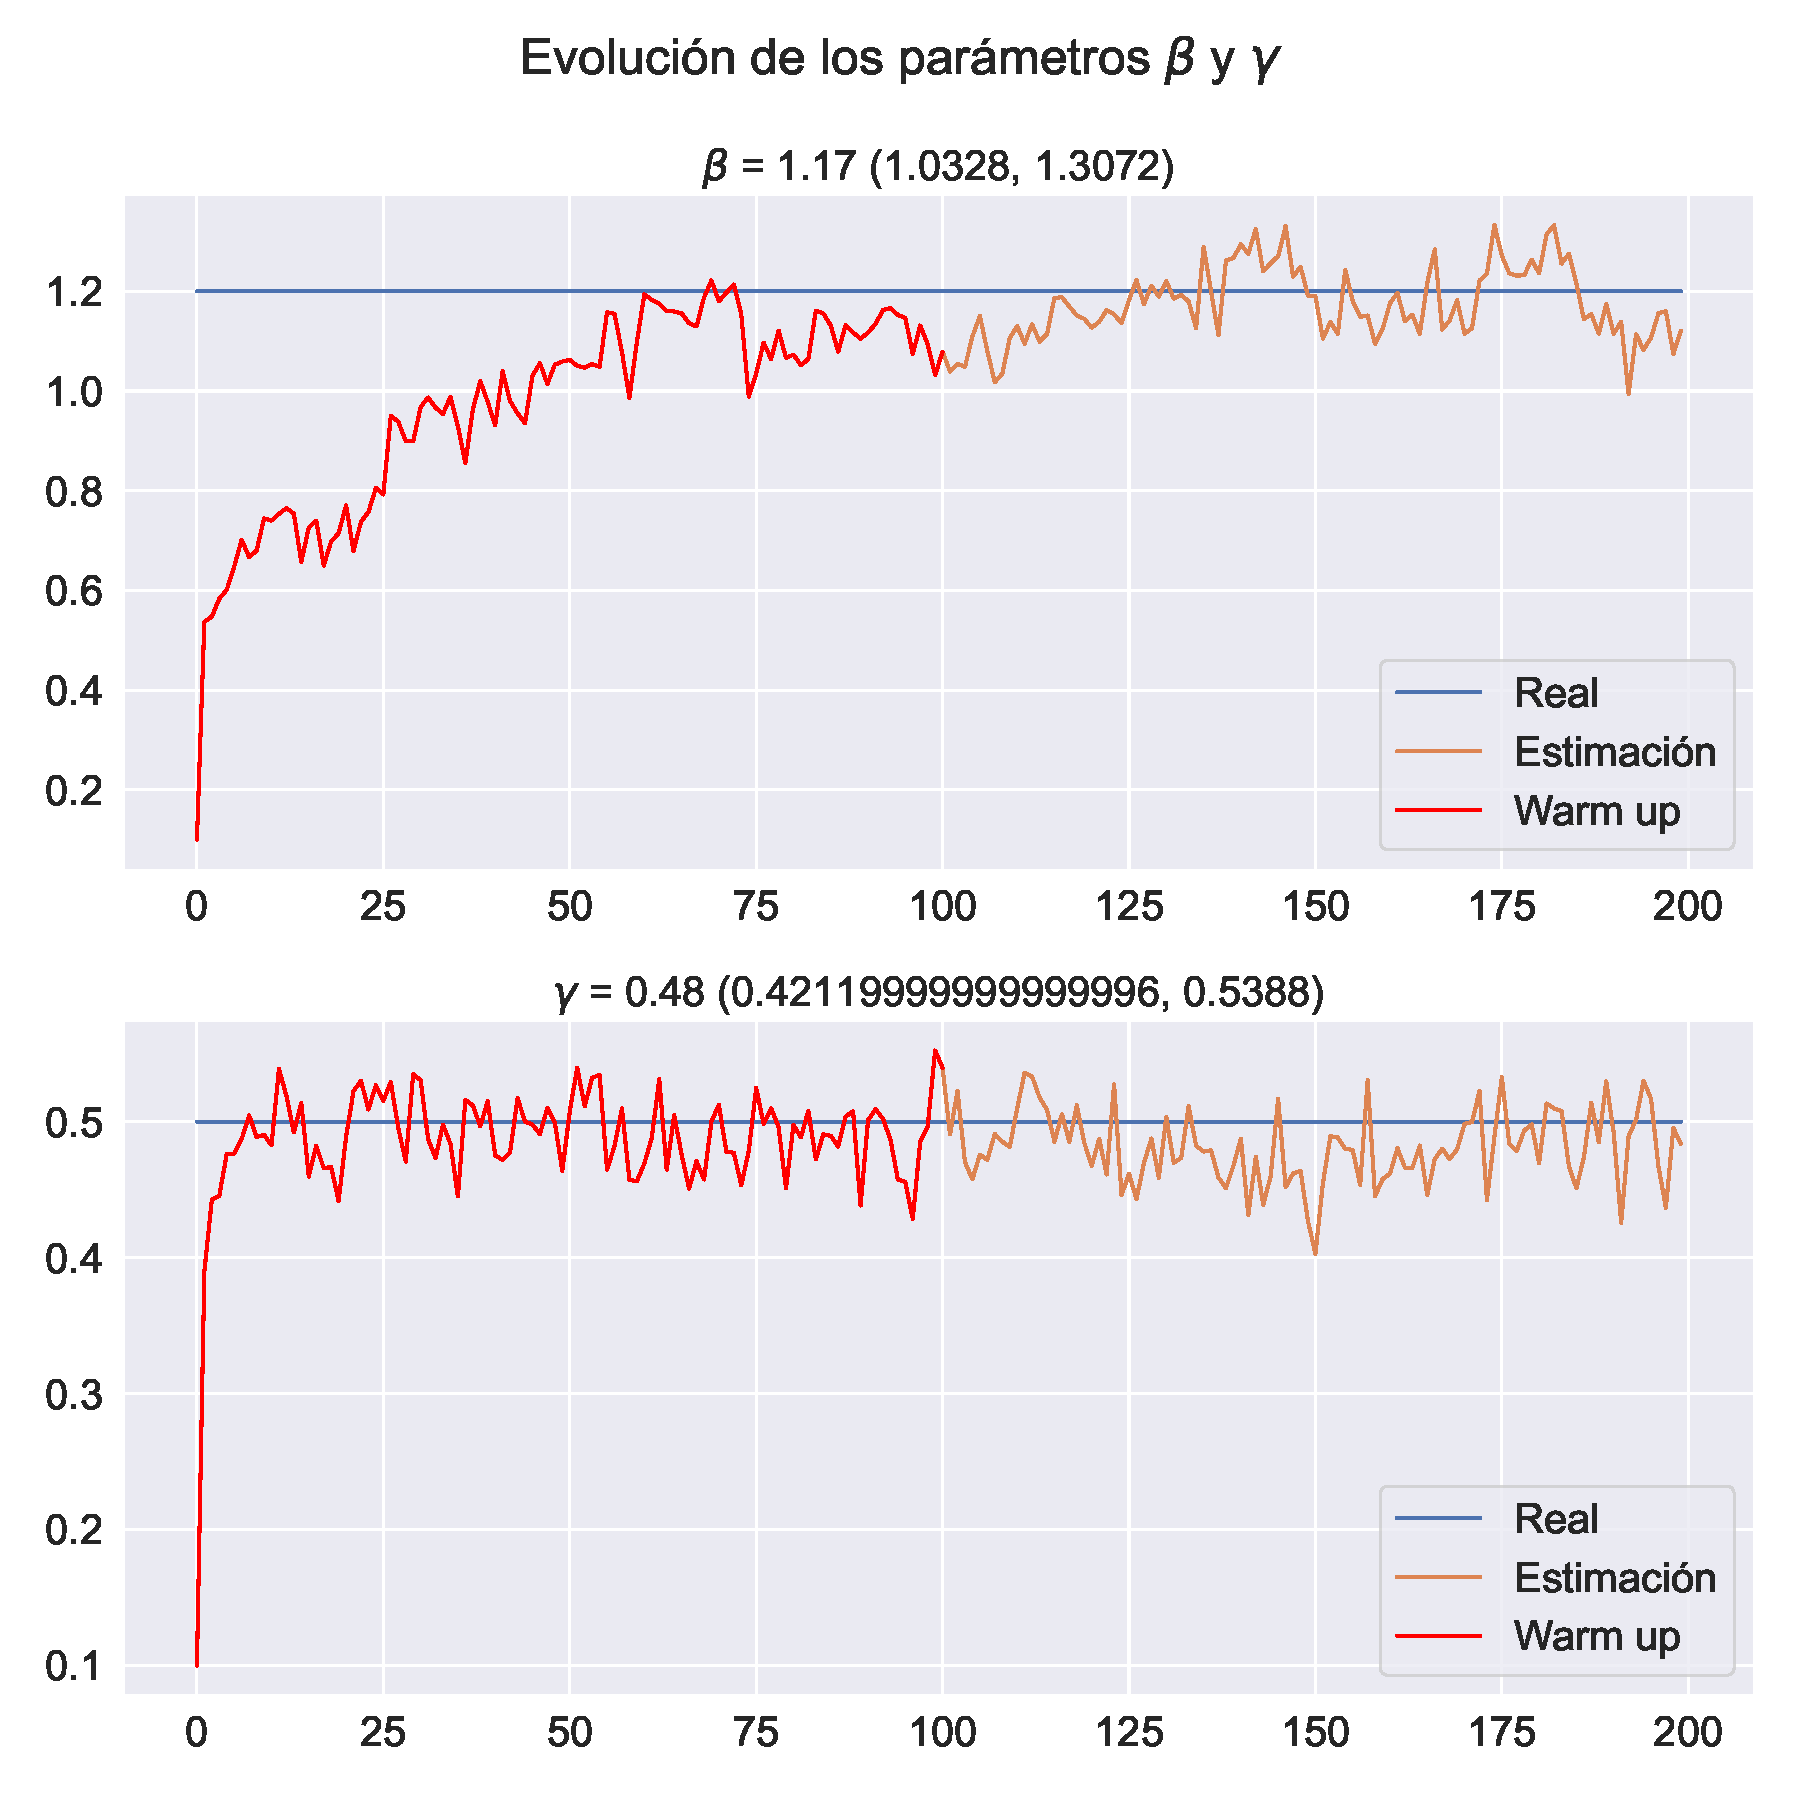
\includegraphics[width=\linewidth]{img/content/chapter4/nonlinear_filters_sir_params_evolution.pdf}
       \caption{}
   \end{subfigure}
    \caption{Resultado para modelo SIR \eqref{eq:SIR}. \\
    (a) Resultado de kerKKF con condición inicial dada por la última iteración del algoritmo de estimación de parámetros, en la primera cadena. \\
    (b) Evolución de la estimación de los parámetros a través de las iteraciones del algoritmo de estimación, en la primera cadena. En rojo se observa el régimen de \textit{warm up}, que son iteraciones no contabilizadas para el valor final, mientras que en naranja se encuentran las últimas iteraciones que sí seran consideradas. En azul se encuentra el valor real del parámetro.}
    \label{fig:param_estim_SIR}
\end{figure}

\begin{figure}[h]
    \centering
    \begin{subfigure}[b]{0.49\textwidth}
         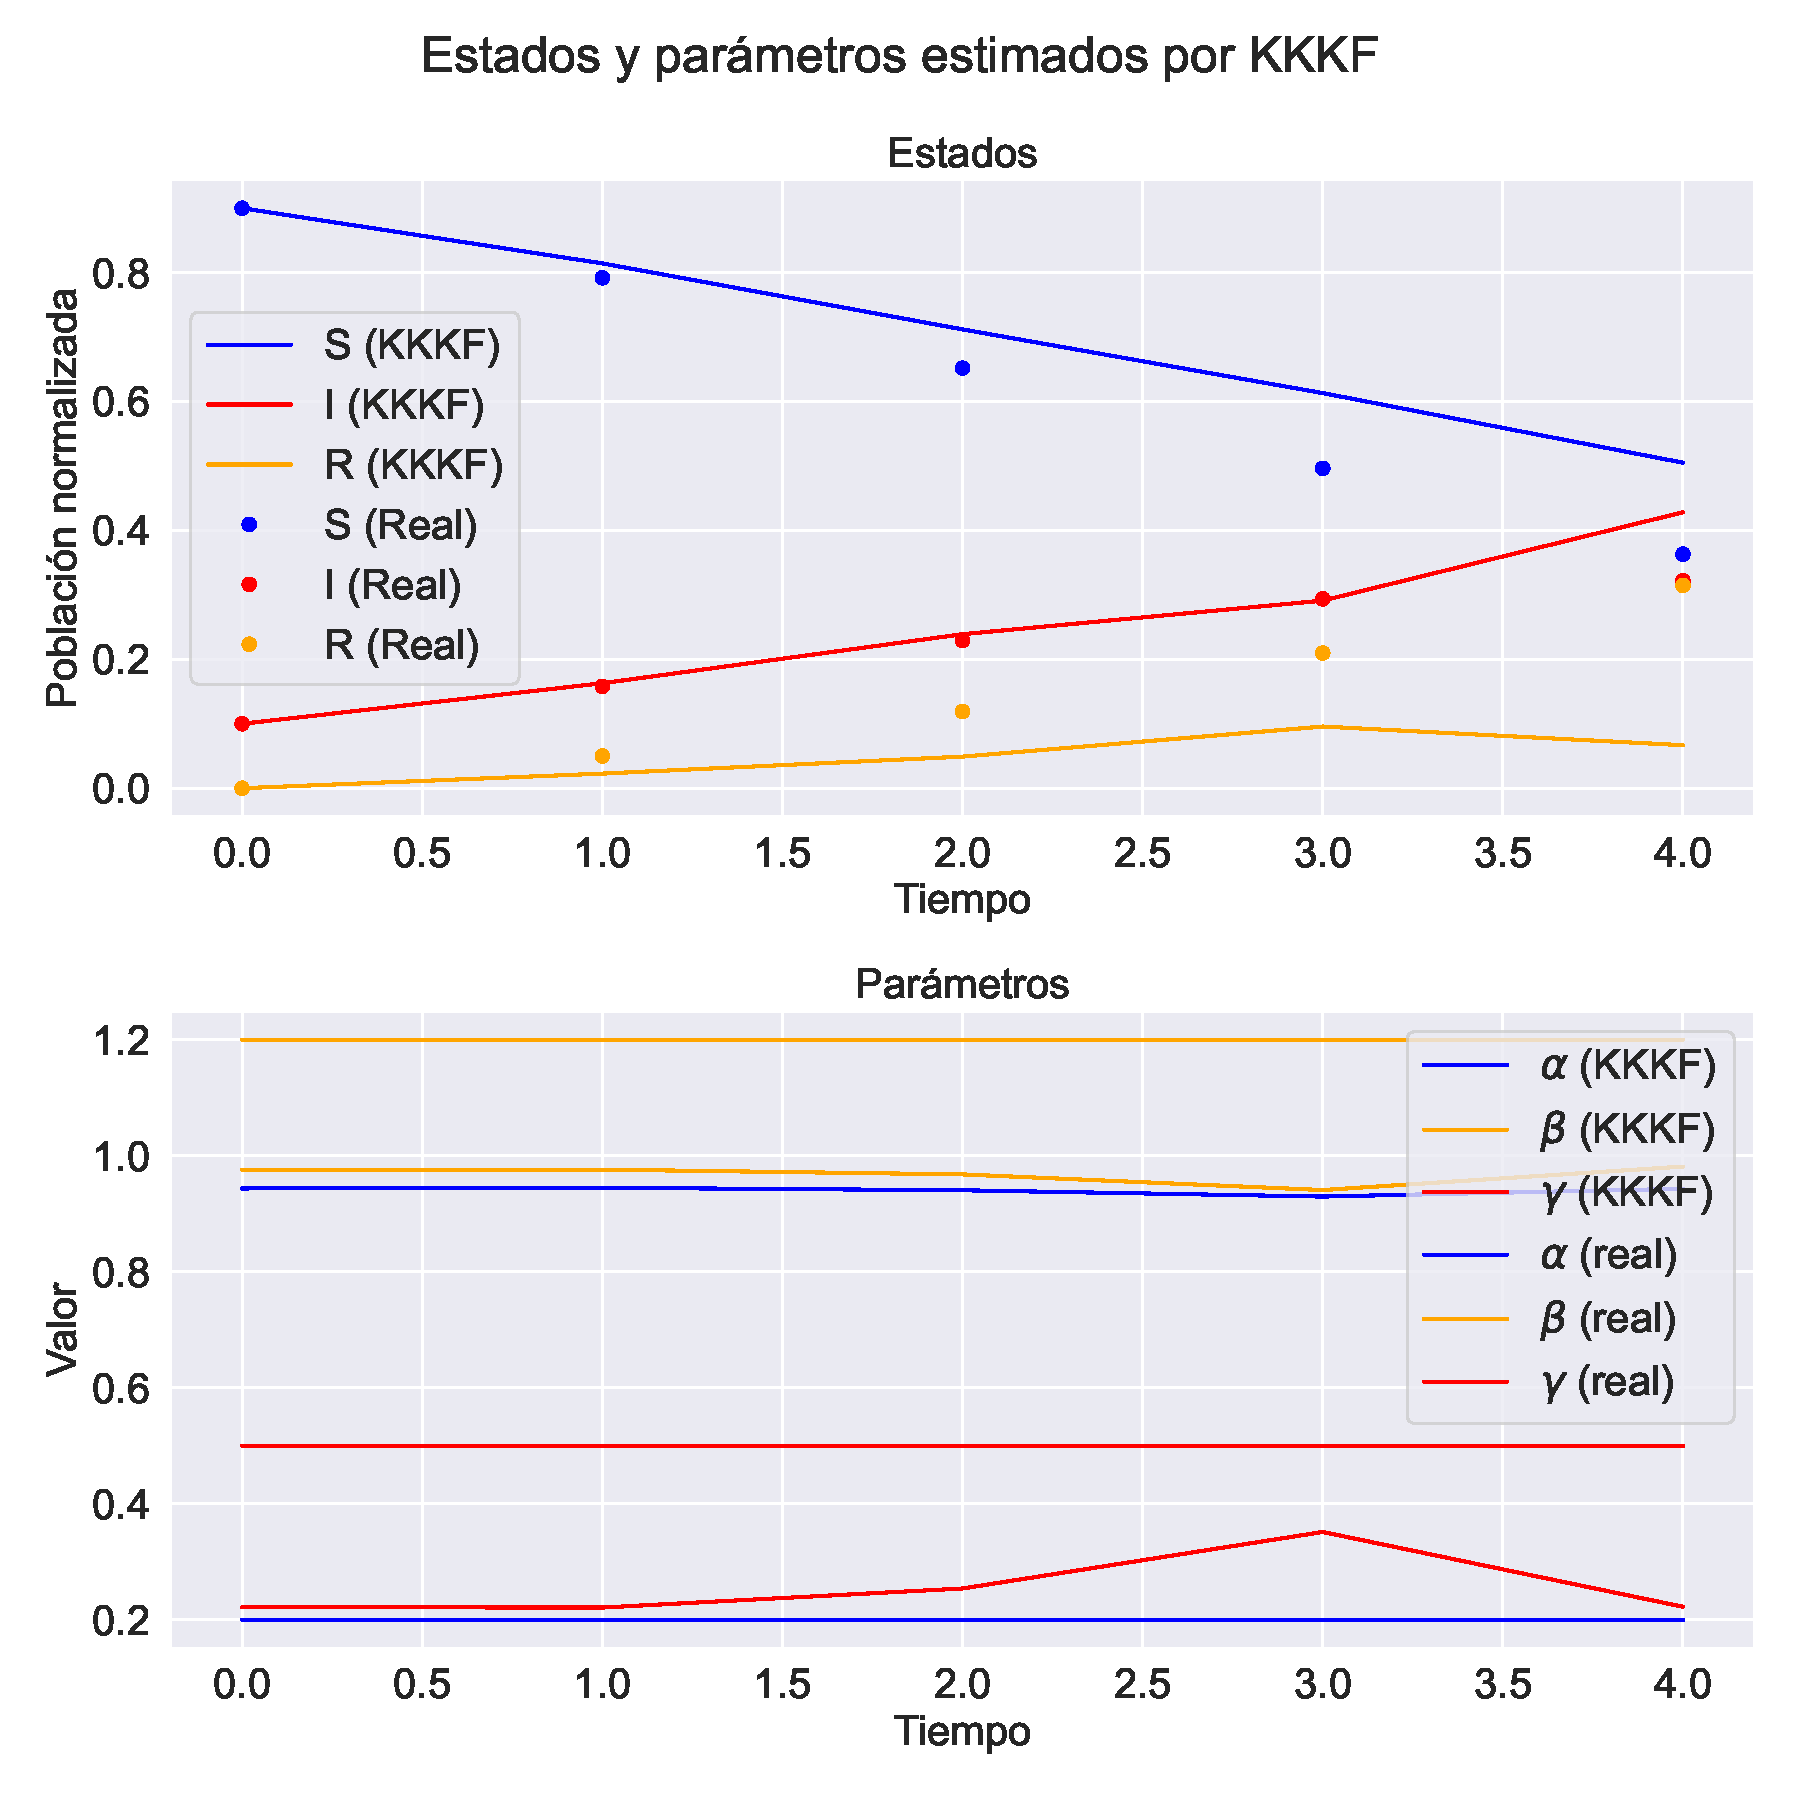
\includegraphics[height=\linewidth]{img/content/chapter4/nonlinear_filters_sir_rec_params.pdf}
         \caption{}
         \label{fig:nonlinear_filters_sir_rec_params}
    \end{subfigure}
    \begin{subfigure}[b]{0.49\textwidth}
         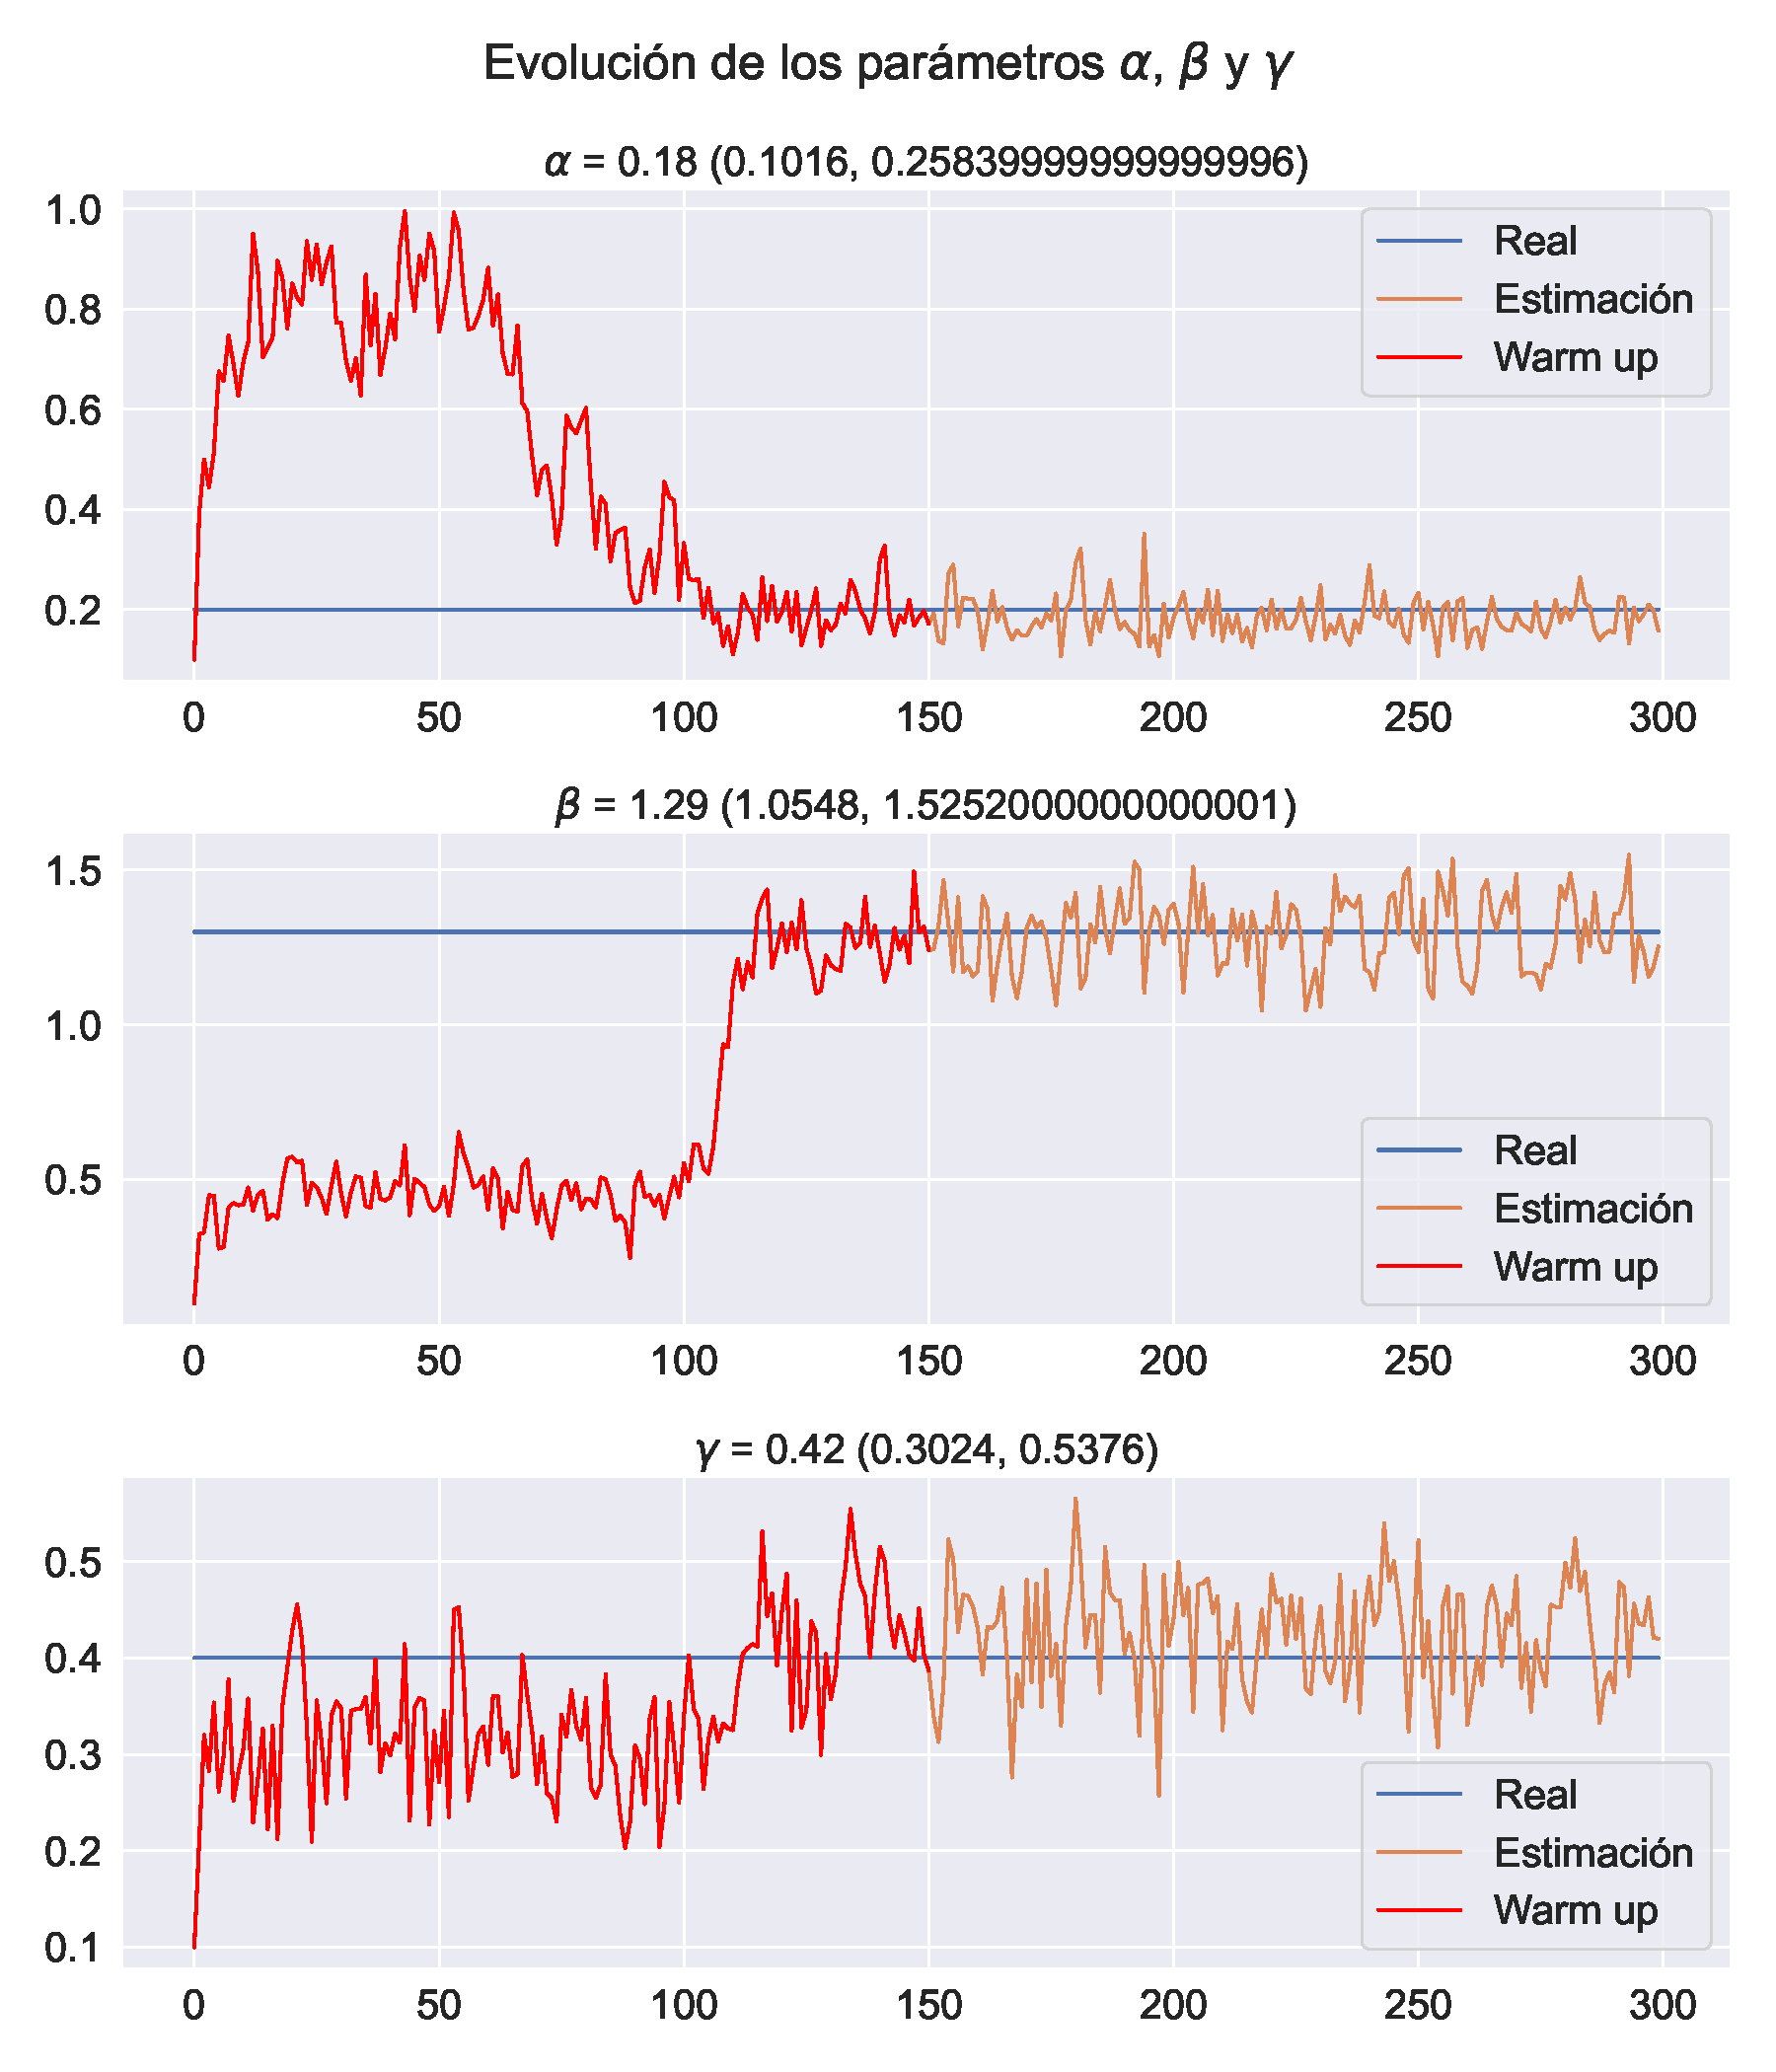
\includegraphics[height=\linewidth]{img/content/chapter4/nonlinear_filters_sir_rec_params_evolution.pdf}
         \caption{}
         \label{fig:nonlinear_filters_sir_rec_params_evolution}
    \end{subfigure}
    \caption{(a) Resultado de kerKKF con condición inicial dada por la última iteración del algoritmo de estimación de parámetros, en la primera cadena, esto para el modelo SIR con pérdida de inmunidad \eqref{eq:SIR_rec}.\\
    (b) Evolución de la estimación de los parámetros del modelo SIR con pérdida de inmunidad \eqref{eq:SIR_rec} a través de las iteraciones del algoritmo de estimación, en la primera cadena. En rojo se observa el régimen de \textit{warm up}, mientras que en naranja se encuentran las iteraciones consideradas para estimación. En azul se encuentra el valor real del parámetro.}
    \label{fig:SIR_inmun}
\end{figure}

\begin{figure}[h]
    \centering
    \begin{subfigure}[b]{0.8\textwidth}
        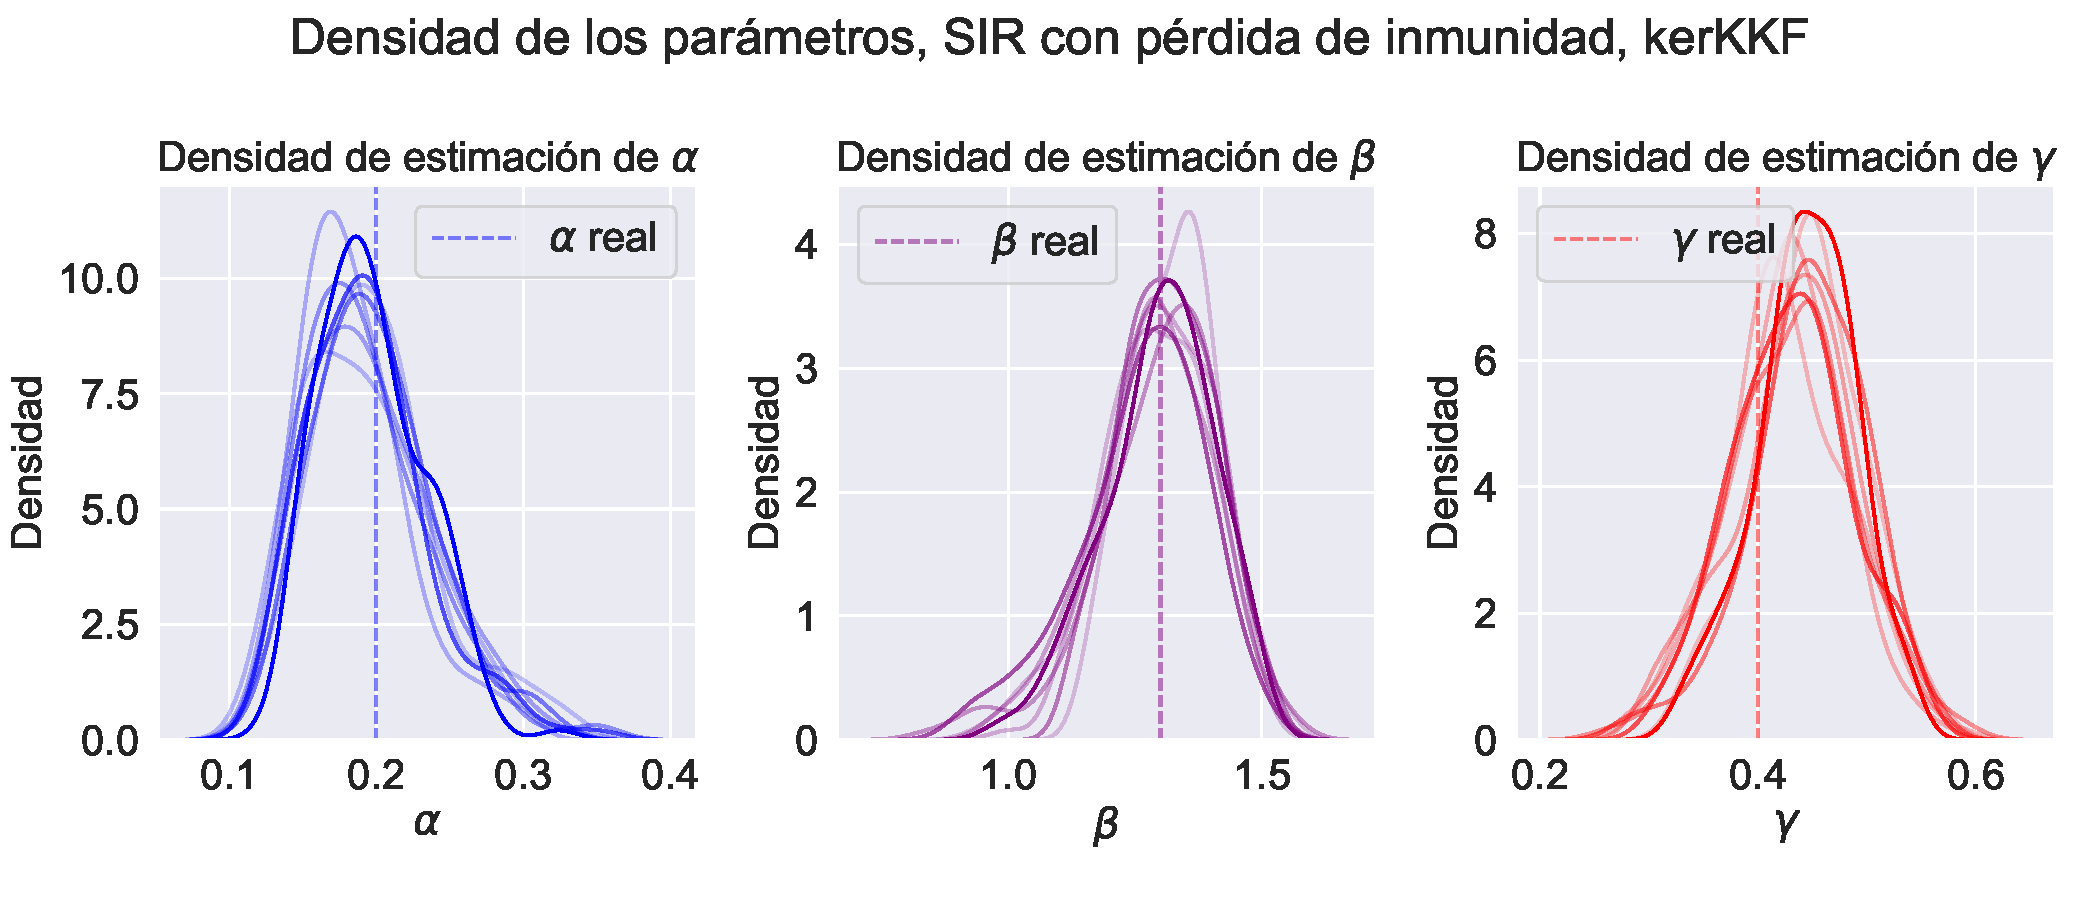
\includegraphics[width=\linewidth]{img/content/chapter4/nonlinear_filters_sir_rec_params_density.pdf}
    \caption{}
    \label{fig:nonlinear_filters_sir_rec_params_density}
    \end{subfigure}
    \begin{subfigure}[b]{0.8\textwidth}
        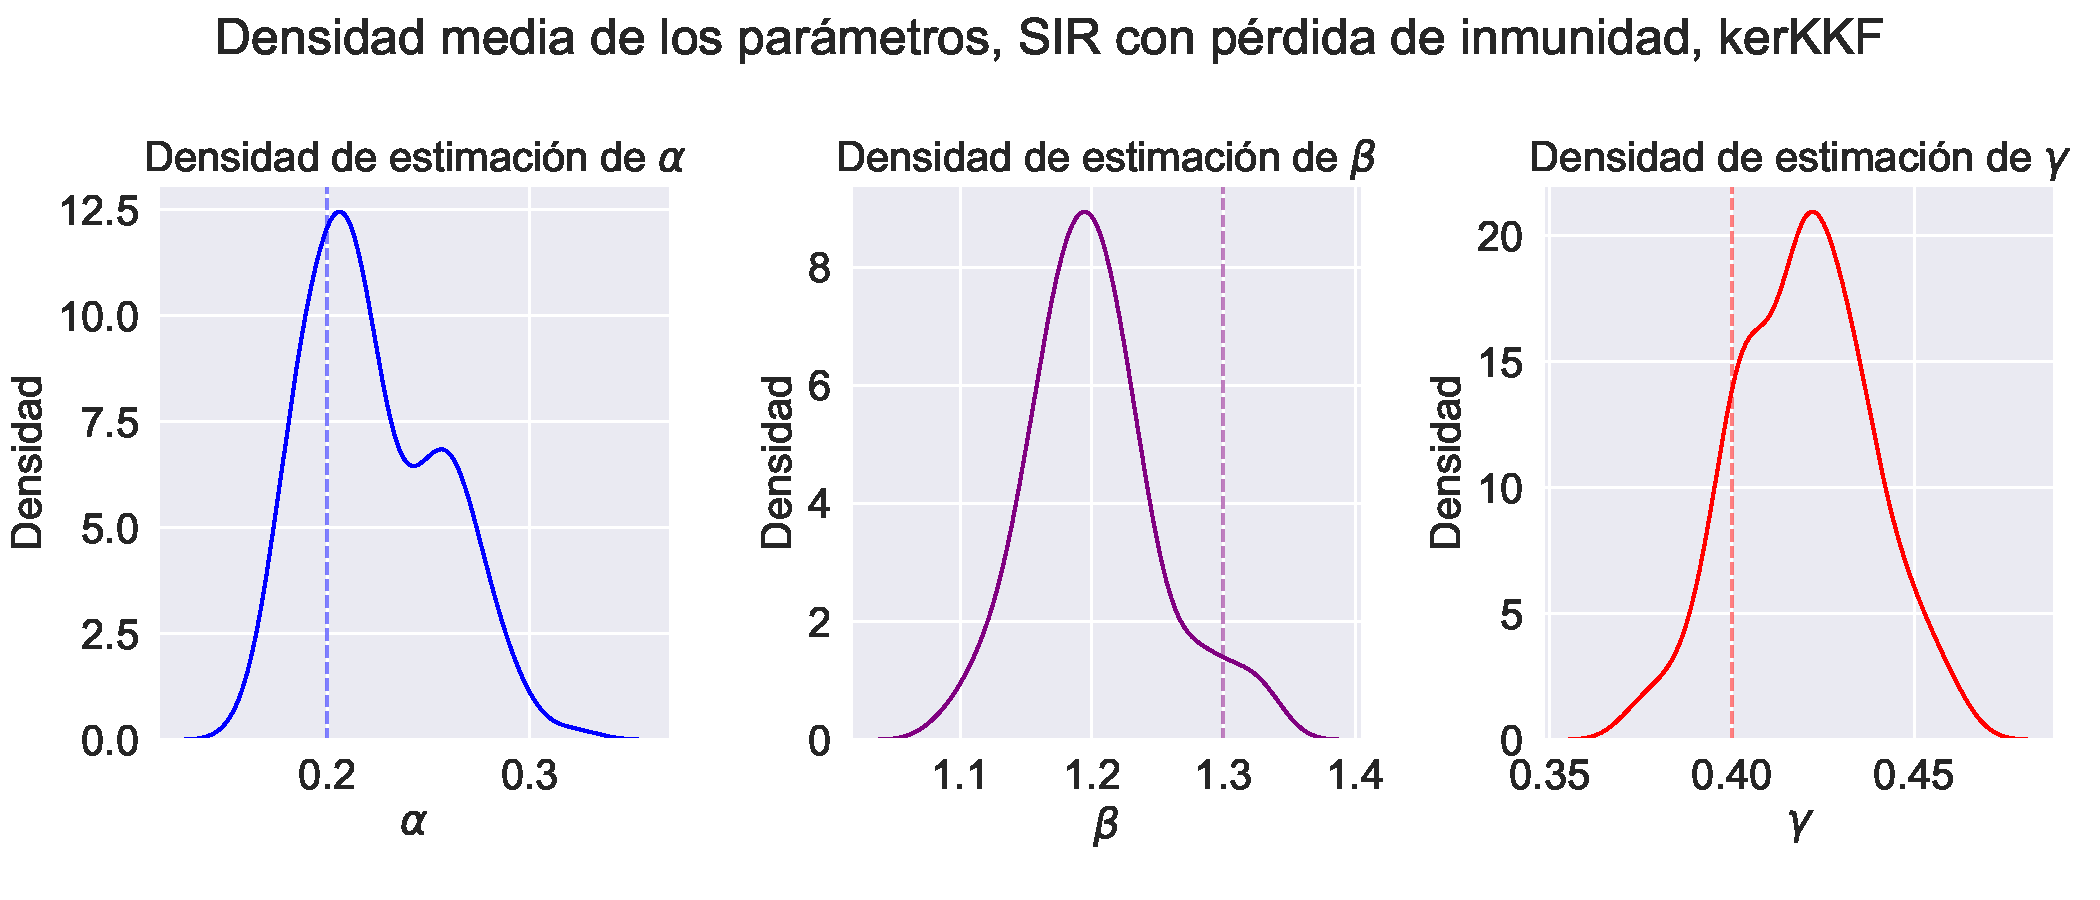
\includegraphics[width=\linewidth]{img/content/chapter4/nonlinear_filters_sir_rec_params_density_mean.pdf}
    \caption{}
    \label{fig:nonlinear_filters_sir_rec_params_density_mean}
    \end{subfigure}
    \caption{A la izquierda el resultado para $\alpha$, al medio para $\beta$ y a la derecha para $\gamma$, parámetros del modelo SIR con pérdida de inmunidad \eqref{eq:SIR_rec}. En línea punteada vertical se encuentra el valor real del parámetro. \\
    (a) Densidades de probabilidad creadas por cada cadena solo considerando las iteraciones posteriores al \textit{warm up}. Por cada una son $8$ densidades correspondientes a cada cadena. \\
    (b) Densidades de probabilidad resultante de promediar las $8$ densidades creadas por cada cadena.}
\end{figure}

\section{Comparación con métodos de Markov Chain Monte Carlo}

\begin{figure}[h]
    \centering
    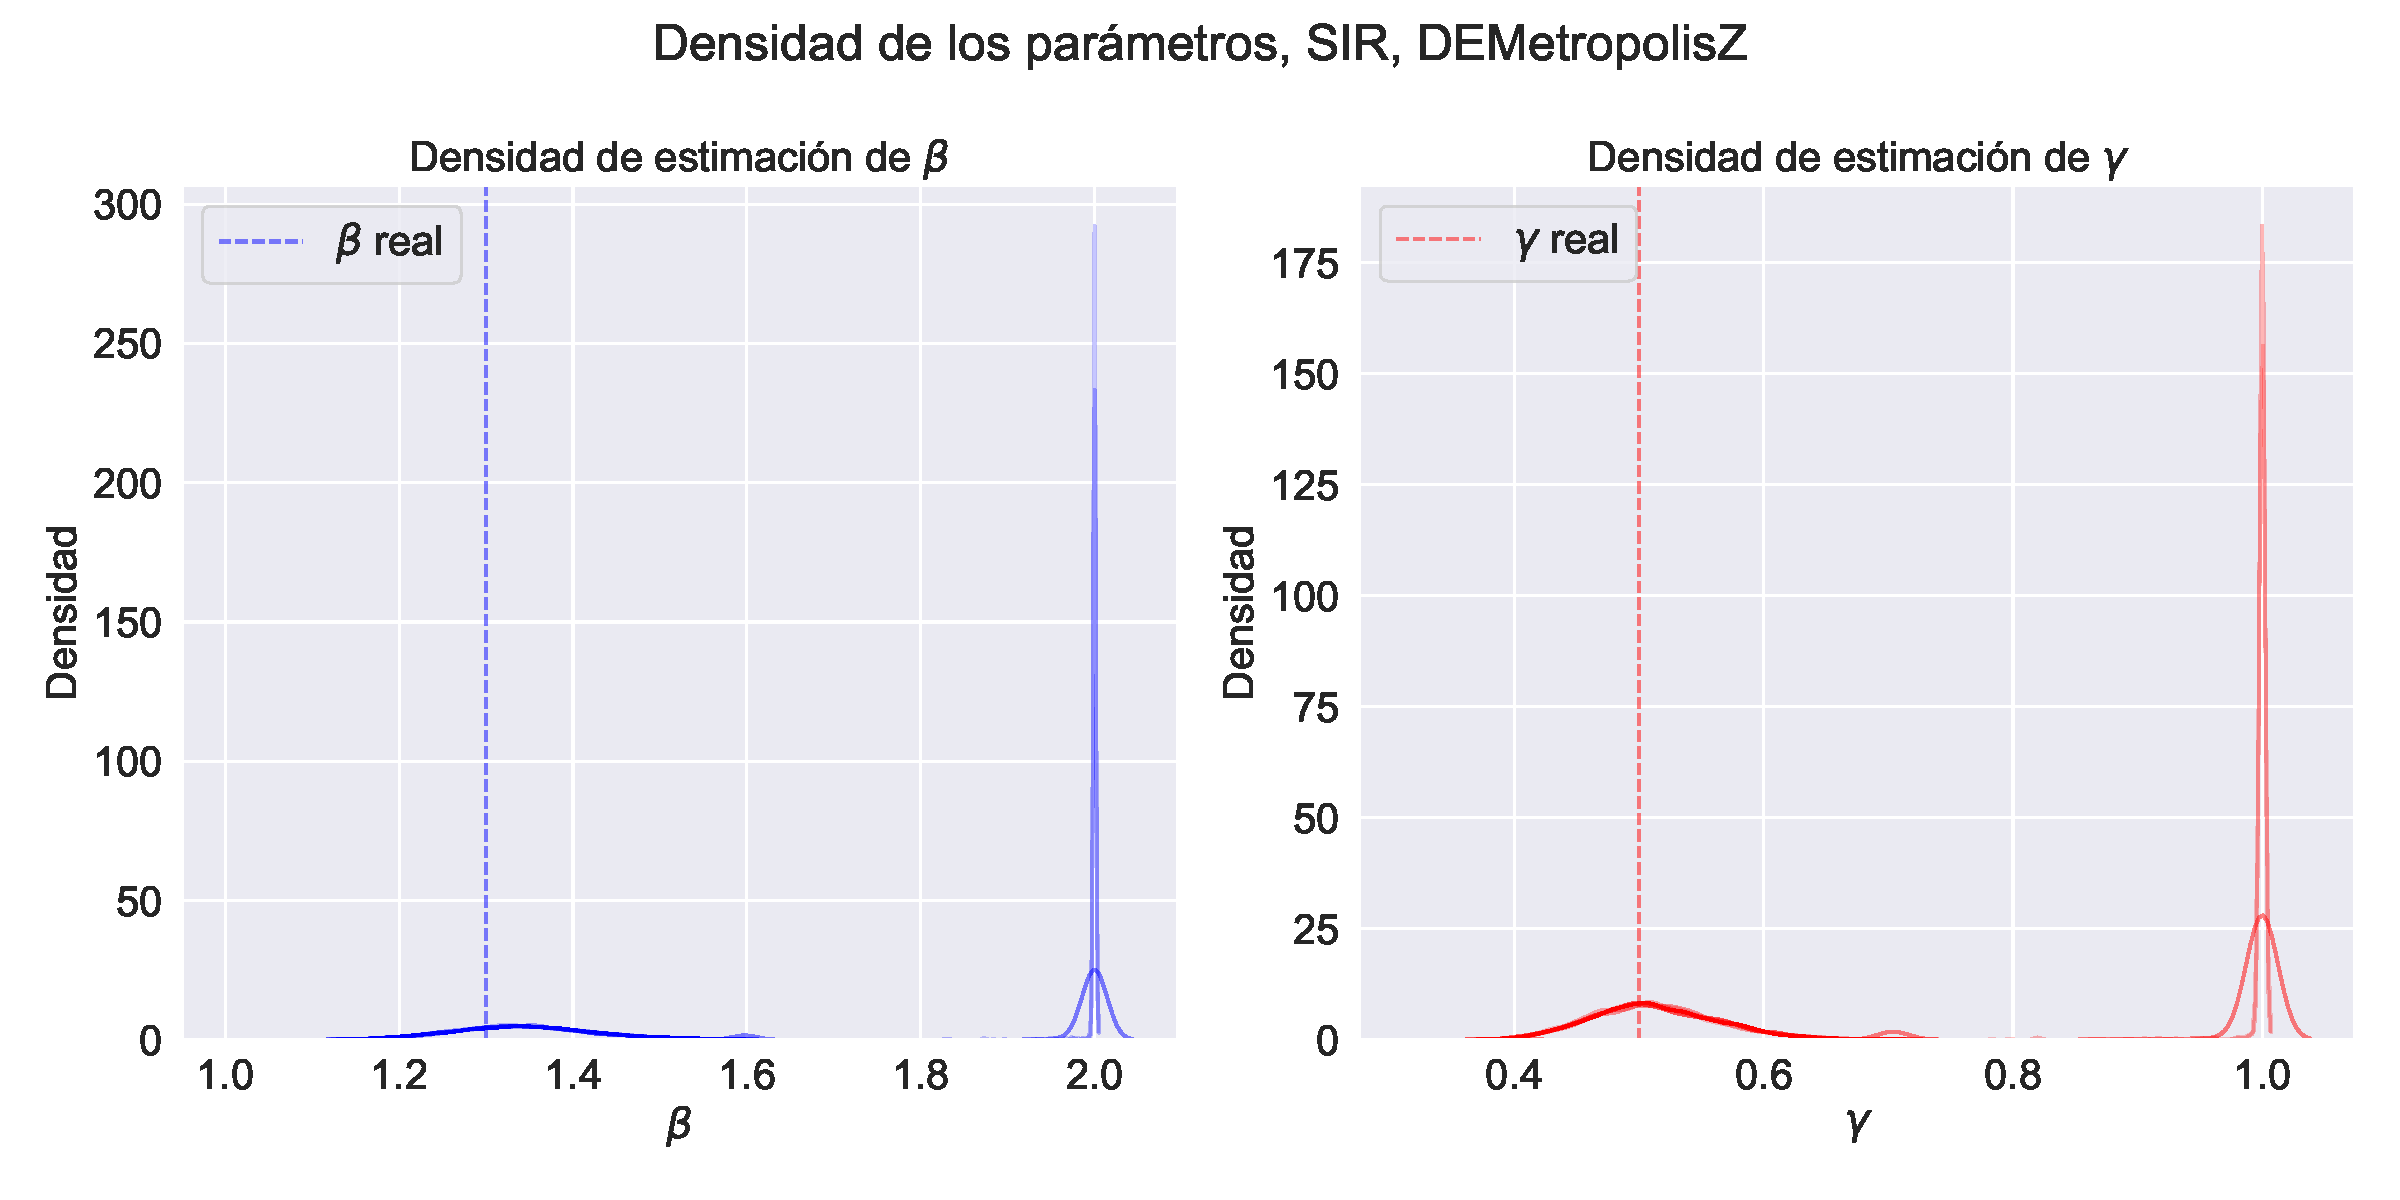
\includegraphics[width=0.8\linewidth]{img/content/chapter4/DEMetropolis_sir_params_density.pdf}
    \caption{Caption}
    \label{fig:enter-label}
\end{figure}

\begin{figure}[h]
    \centering
    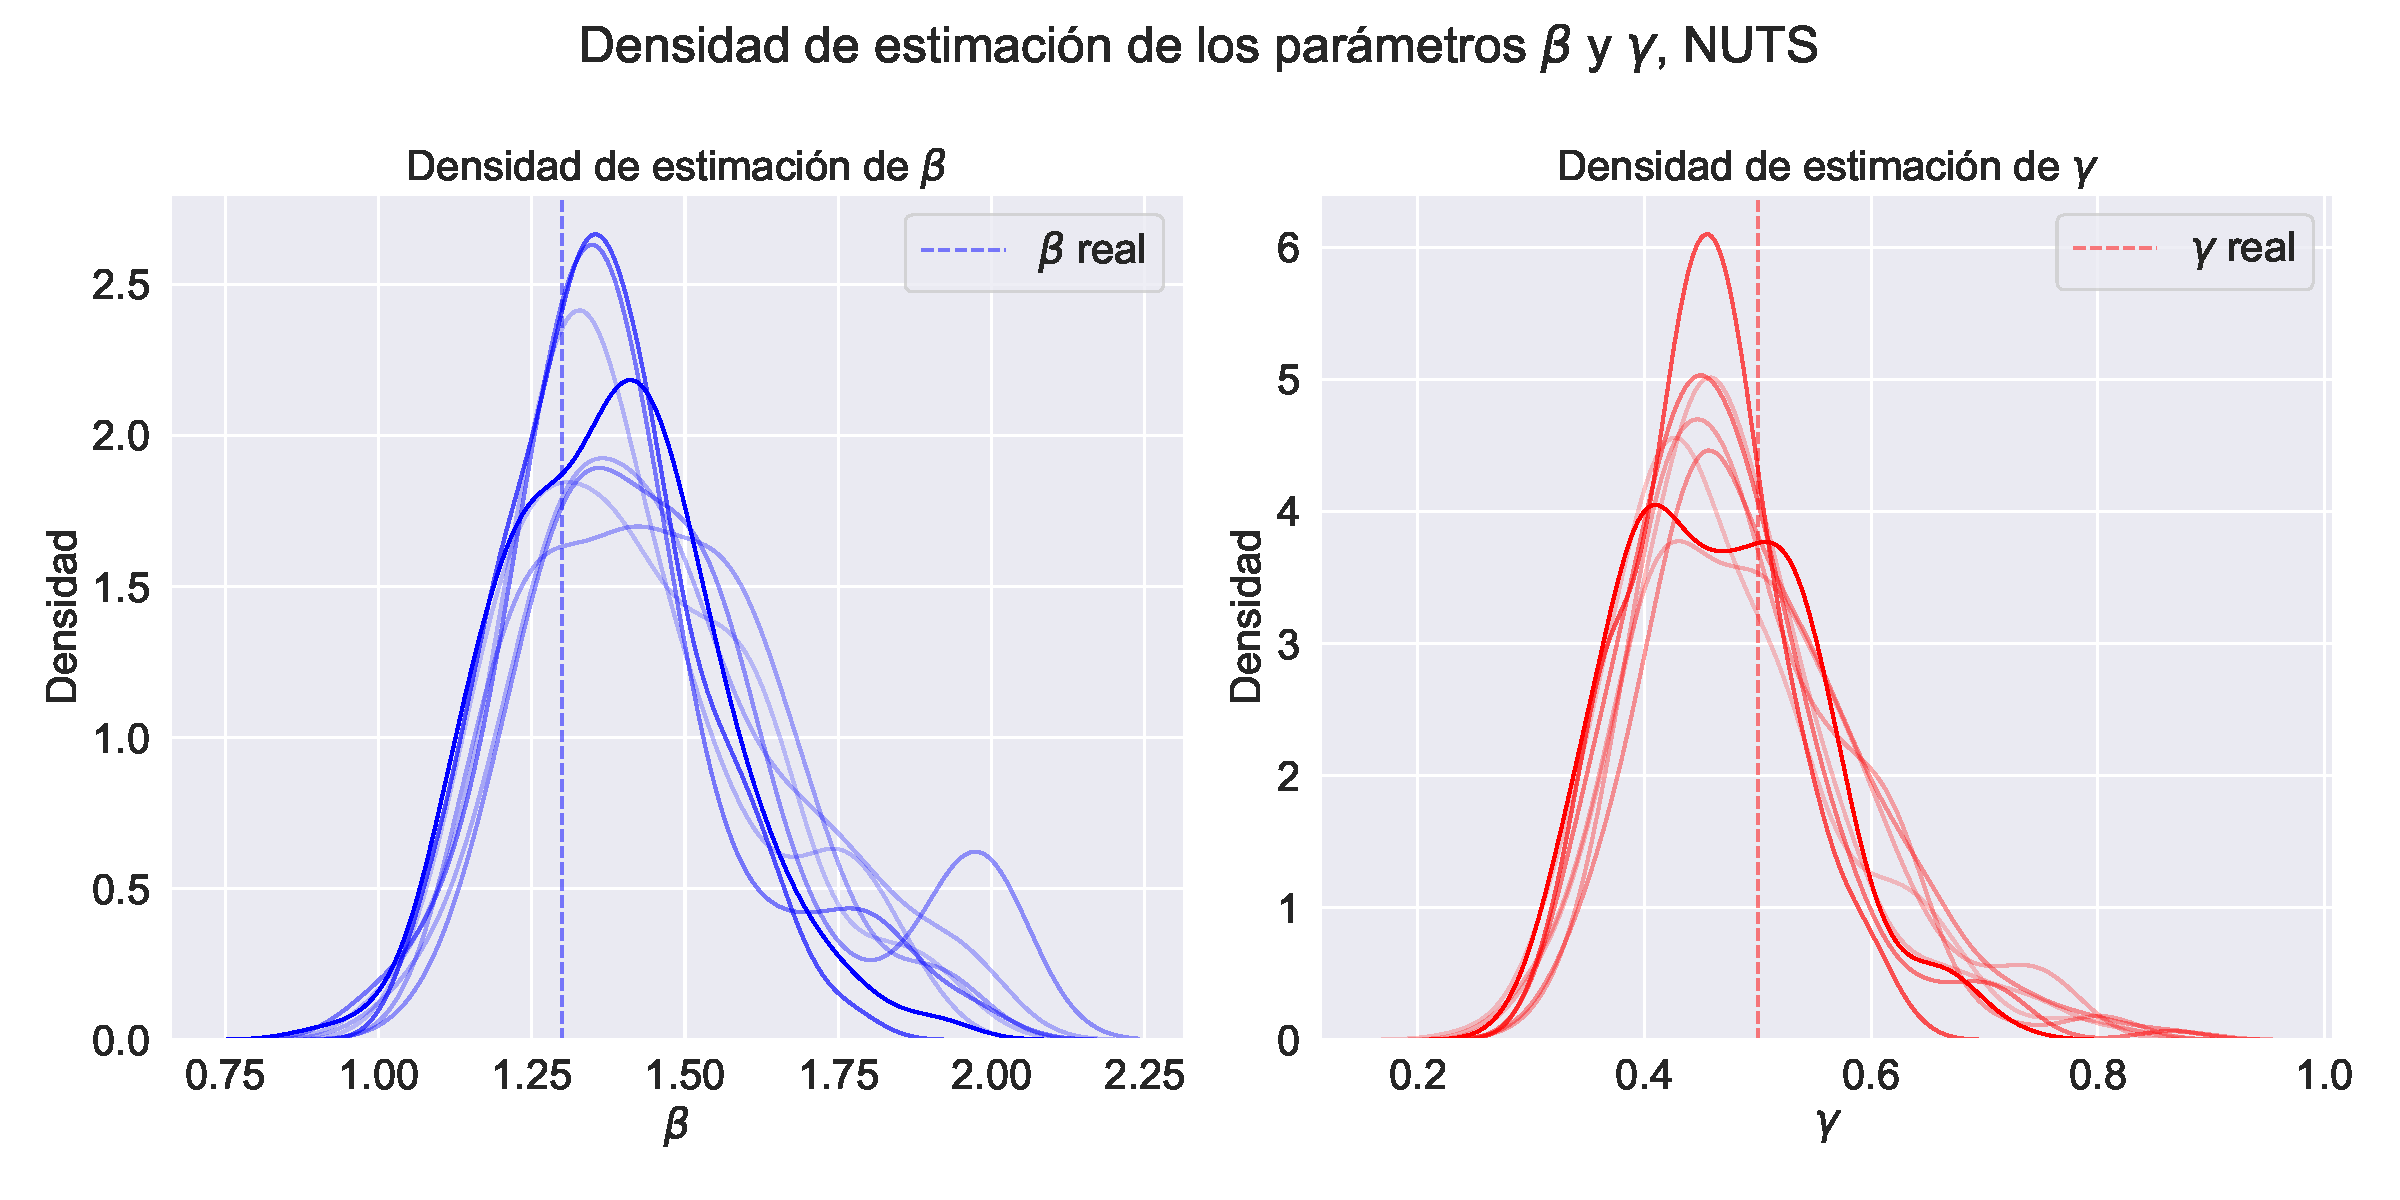
\includegraphics[width=0.8\linewidth]{img/content/chapter4/NUTS_sir_params_density.pdf}
    \caption{Caption}
    \label{fig:enter-label}
\end{figure}

\begin{figure}[h]
    \centering
    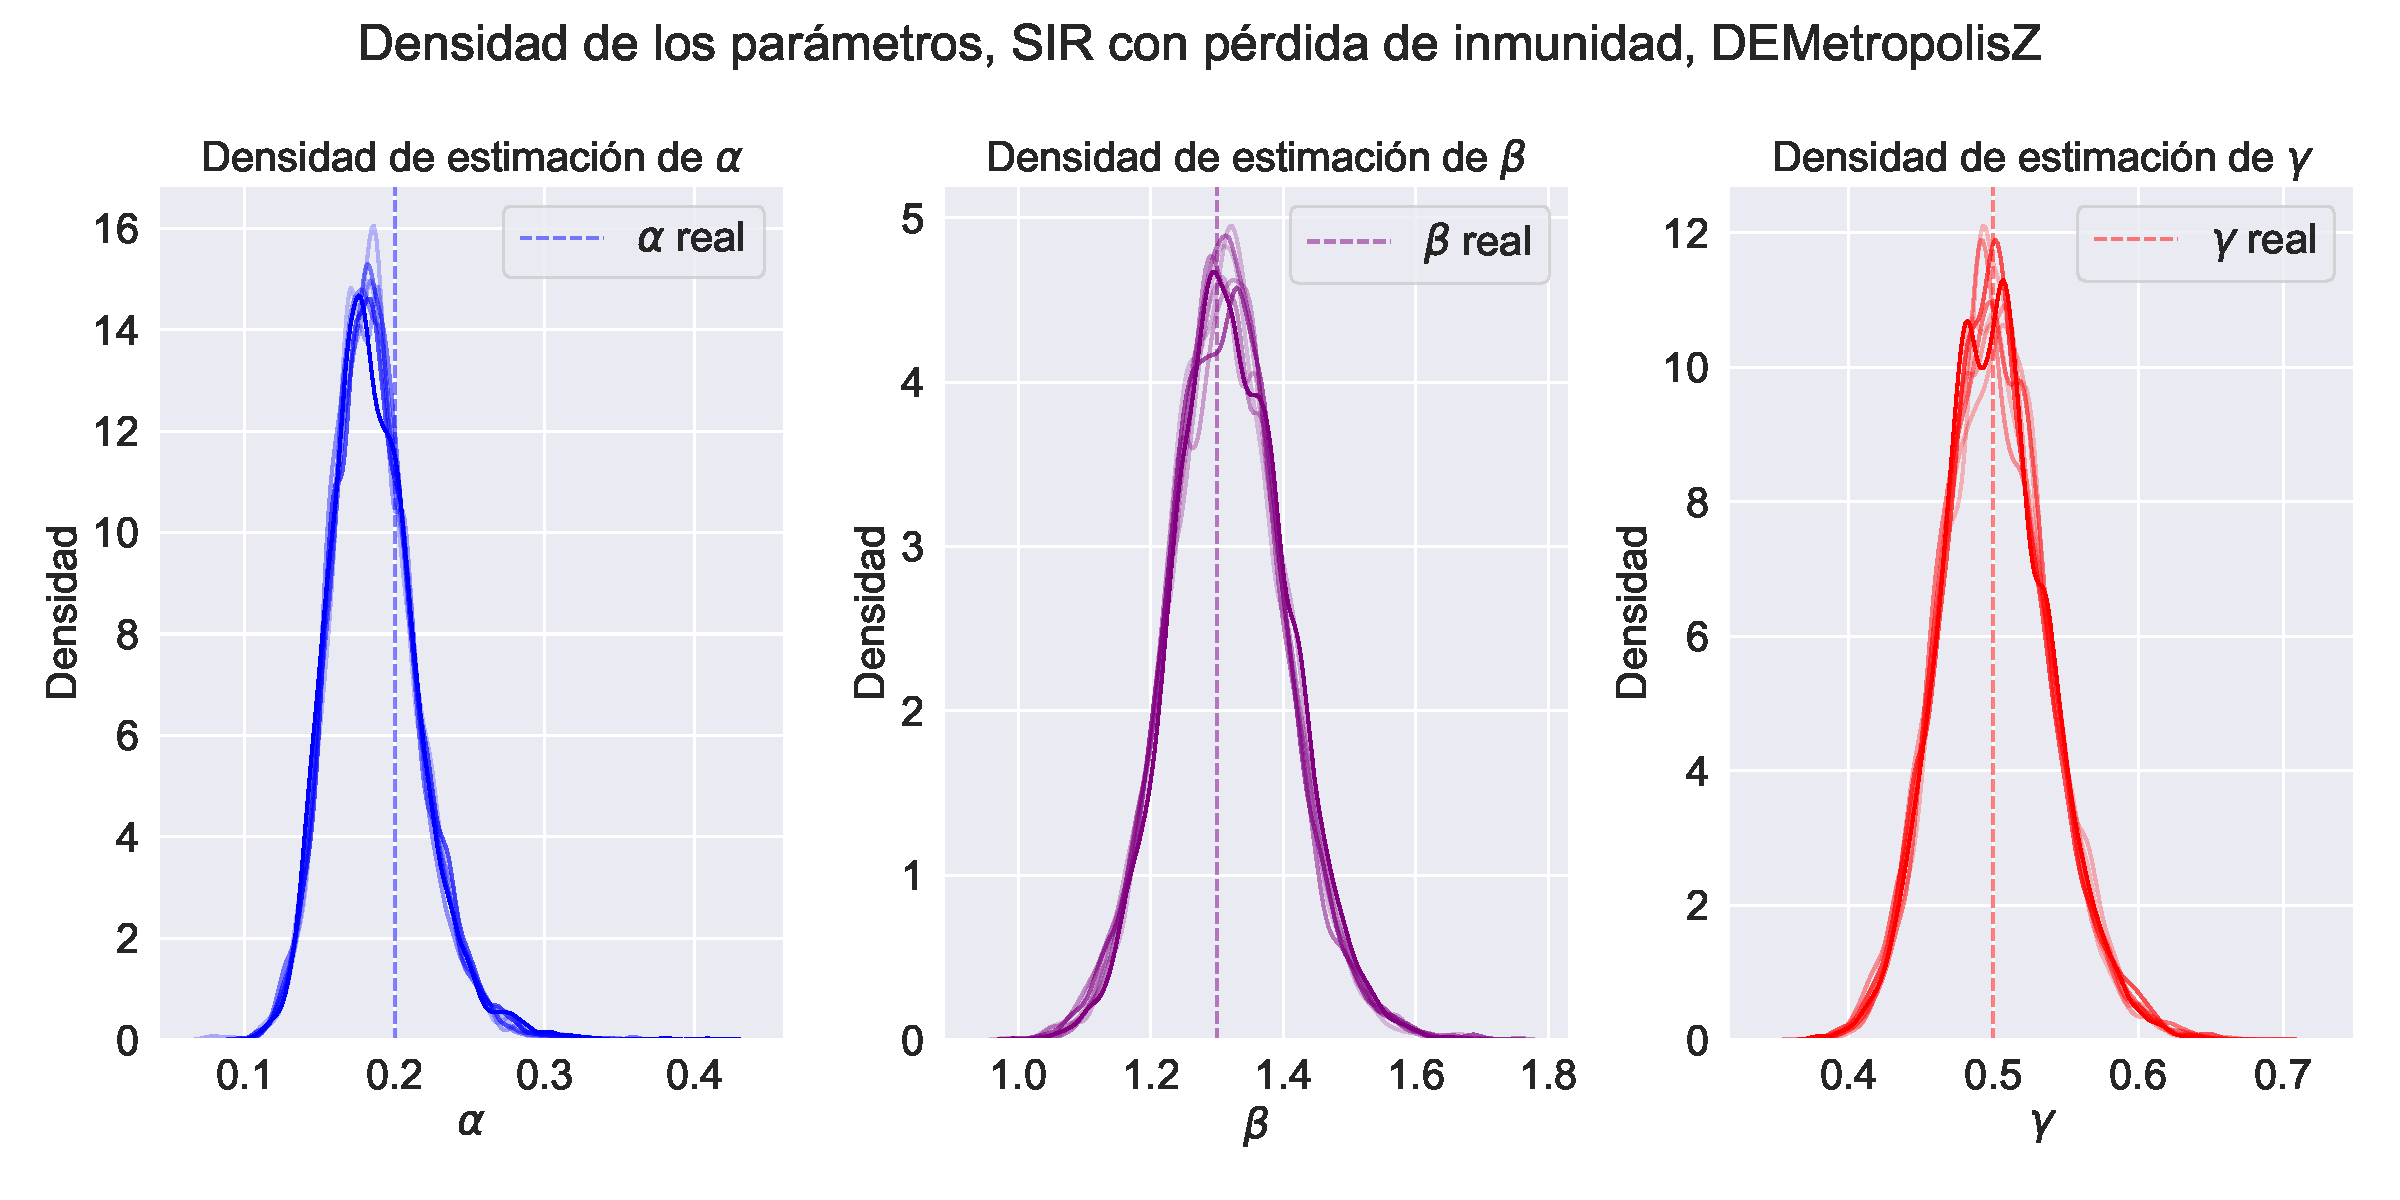
\includegraphics[width=0.8\linewidth]{img/content/chapter4/DEMetropolis_sir_rec_params_density.pdf}
    \caption{Caption}
    \label{fig:enter-label}
\end{figure}

\begin{figure}[h]
    \centering
    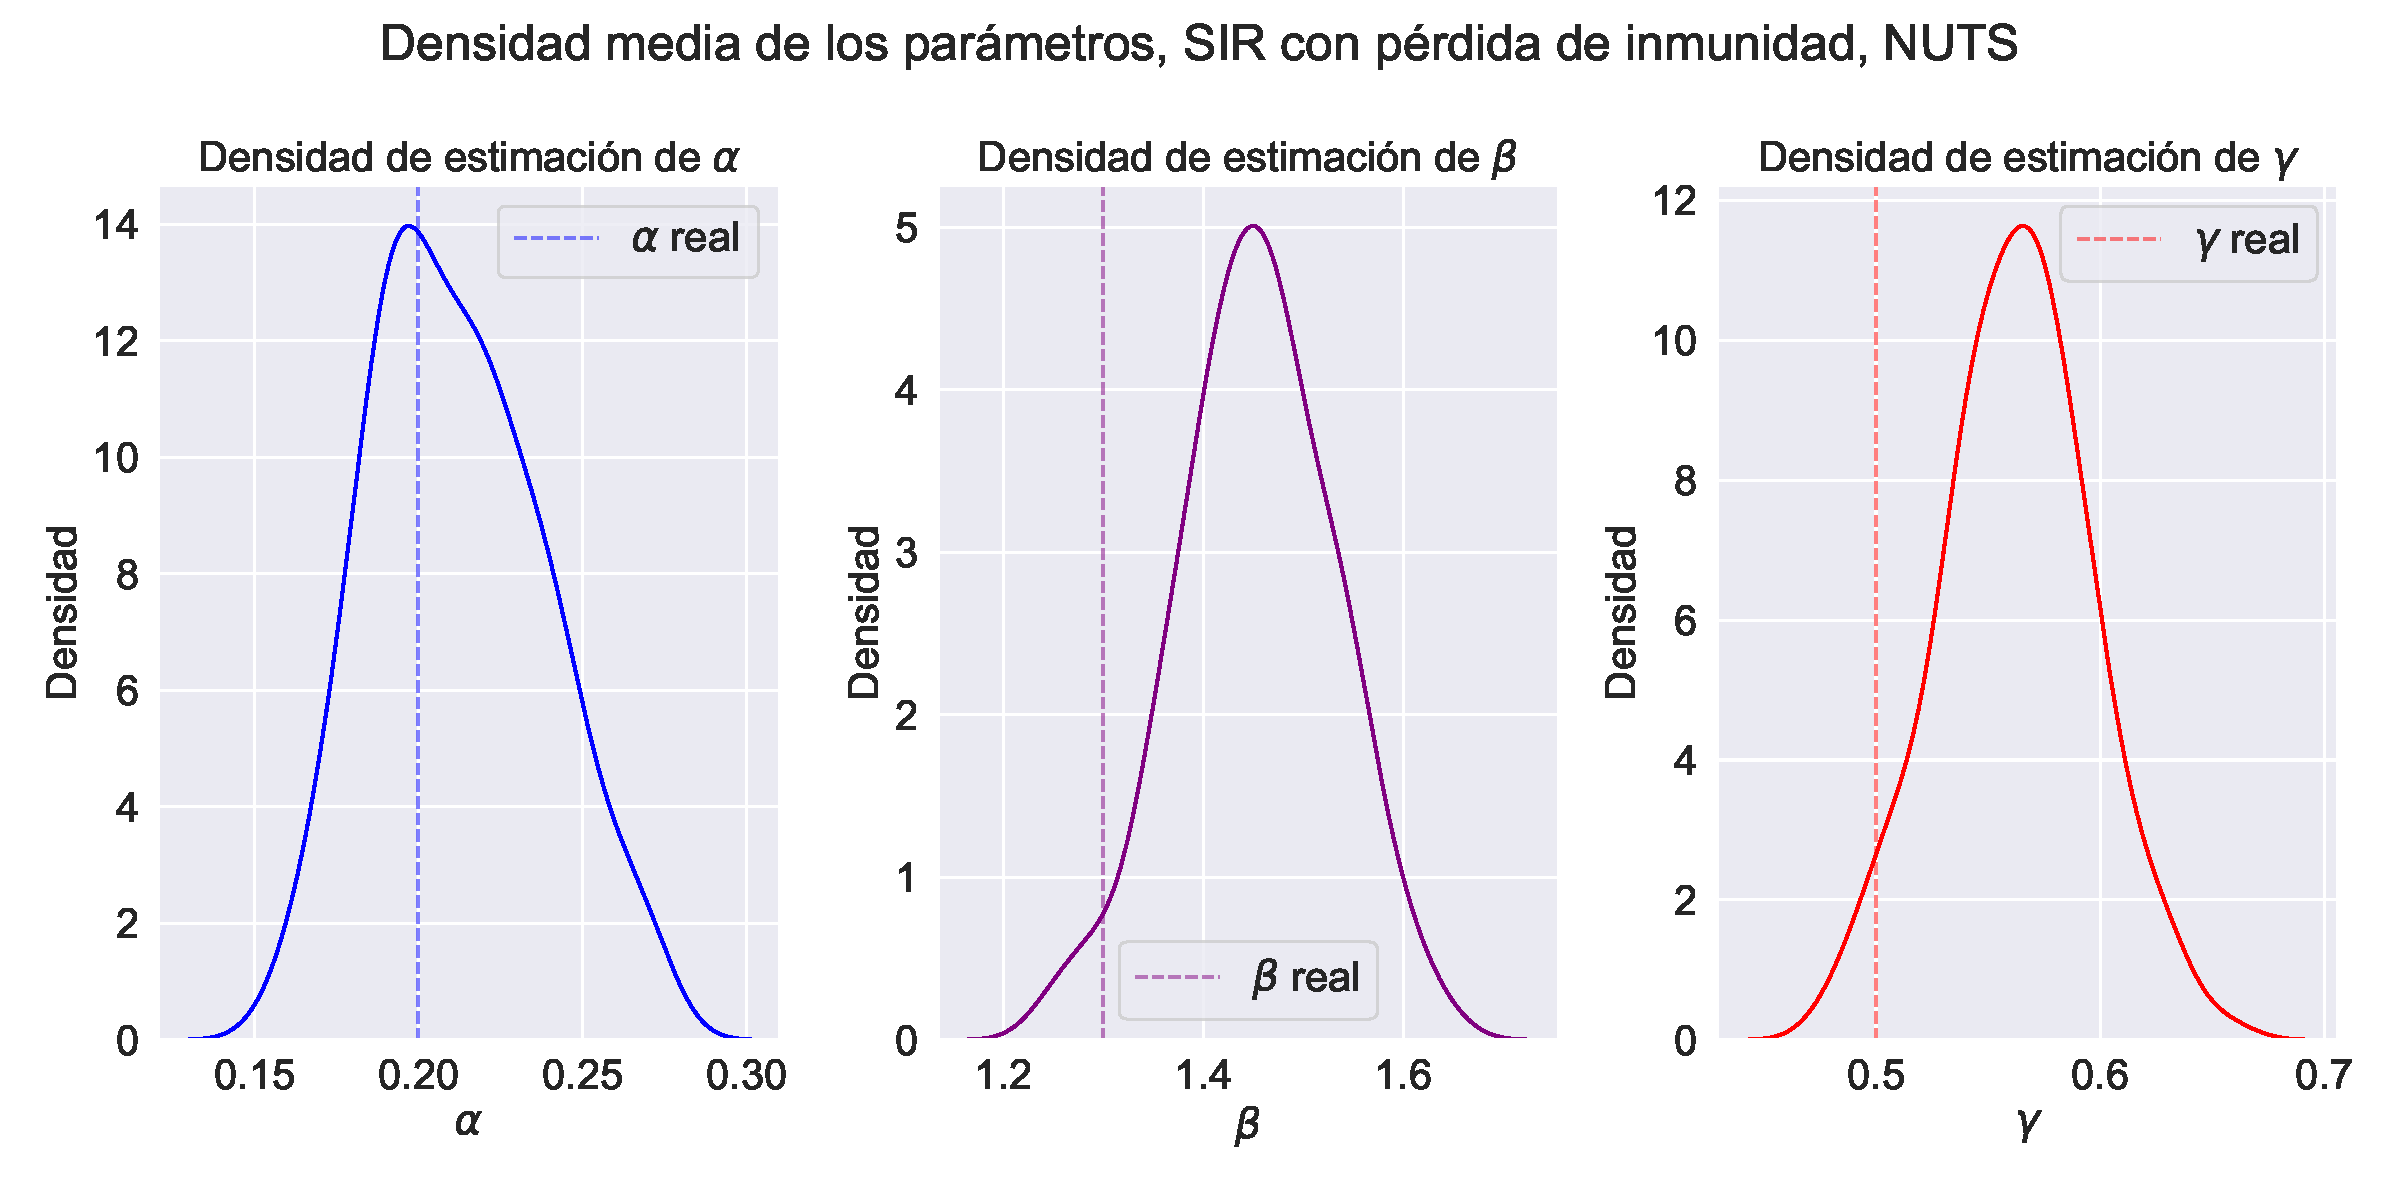
\includegraphics[width=0.8\linewidth]{img/content/chapter4/NUTS_sir_rec_params_density.pdf}
    \caption{Caption}
    \label{fig:enter-label}
\end{figure}
